\documentclass{report}

\usepackage[a4paper,margin=0.5in]{geometry}
\usepackage{array}
\usepackage{xcolor}
\usepackage{graphicx}
\usepackage{float}
\usepackage{adjustbox}

\linespread{1.14}
\renewcommand{\thesection}{\arabic{section}}

\author{Niko Hellgren \texttt{<nipehe@utu.fi>}}
\title{Exercise Work 1\\\large Data Analysis and Knowledge Discovery}

\newcolumntype{P}[1]{>{\raggedleft\arraybackslash}b{#1}}
\newcommand{\bftab}{\fontseries{b}\selectfont}

\begin{document}
\maketitle
\tableofcontents
\newpage

\section{Plots of single attributes}
The subsections of this section contain three figures each and correspond to the features in the data set: one with four histograms of the data set; one with the same histograms but with outliers further than 3 standard deviations from the mean filtered; and one with a boxplot of the feature.

In all of the cases, either Scott's rule or Sturges' rule seemed to give the best binning. Square-root choice produced too many bins every time due to the fixed size on the data set. Freedman-Diaconis' choice gave amounts between Scott's rule's and Square-root choice's ones, but the amount of bins was still too large in most cases.

The histograms were produced by taking the corresponding feature values from the whole set, in case of the filtered version filtered out those further than 3 standard deviations from the mean, calculating the bin amounts using different formulas and plotted the histograms using \textit{matplotlib}'s \texttt{hist} function with the calculated bin count.
\subsection{citric acid}
\begin{figure}[H]
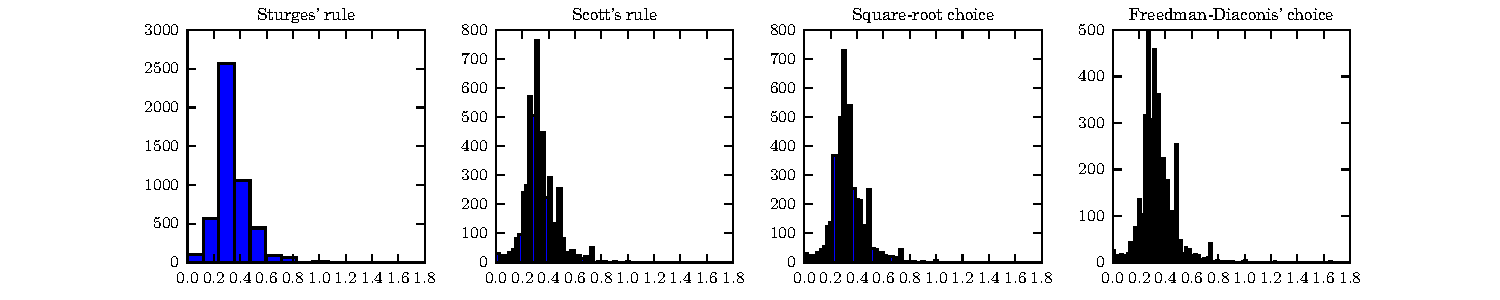
\includegraphics[width=\textwidth]{histograms/citric_acid.pdf}
\caption{Histograms of attribute \emph{citric acid} using different binning methods}\end{figure}

\begin{figure}[H]
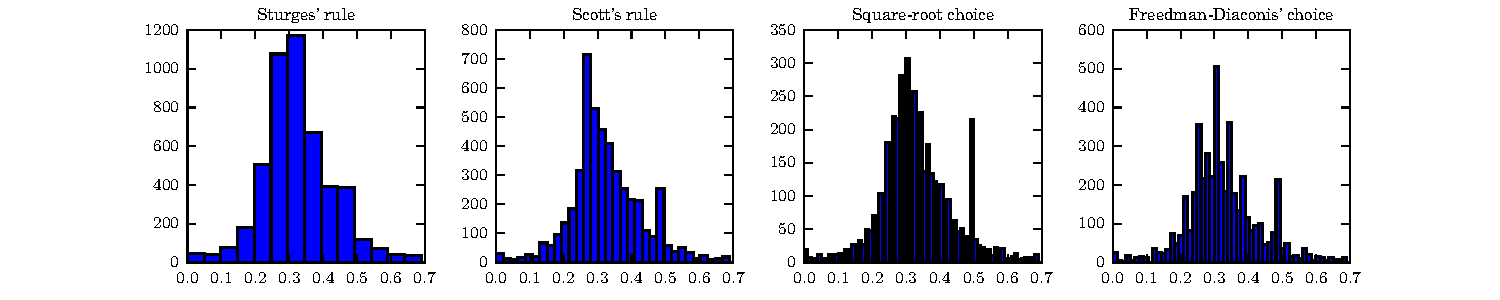
\includegraphics[width=\textwidth]{histograms/citric_acid_filtered.pdf}
\caption{Histograms of attribute \emph{citric acid} with outliers further than 3 standard deviations from the mean filtered}
\end{figure}

\begin{figure}[H]
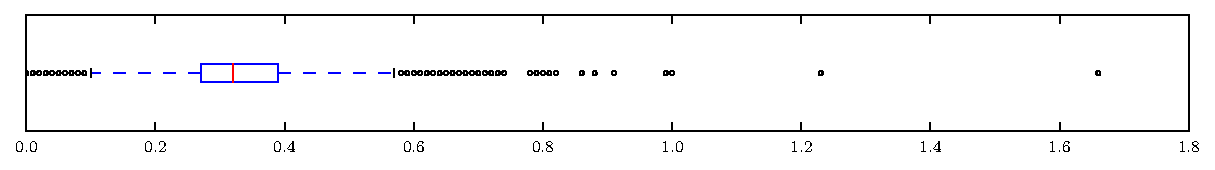
\includegraphics[width=\textwidth]{boxplots/citric_acid.pdf}
\caption{Boxplot of attribute \emph{citric acid}. The values are quite spread and there are a couple of outliers.}\end{figure}

\newpage
\subsection{free sulfur dioxide}
\begin{figure}[H]
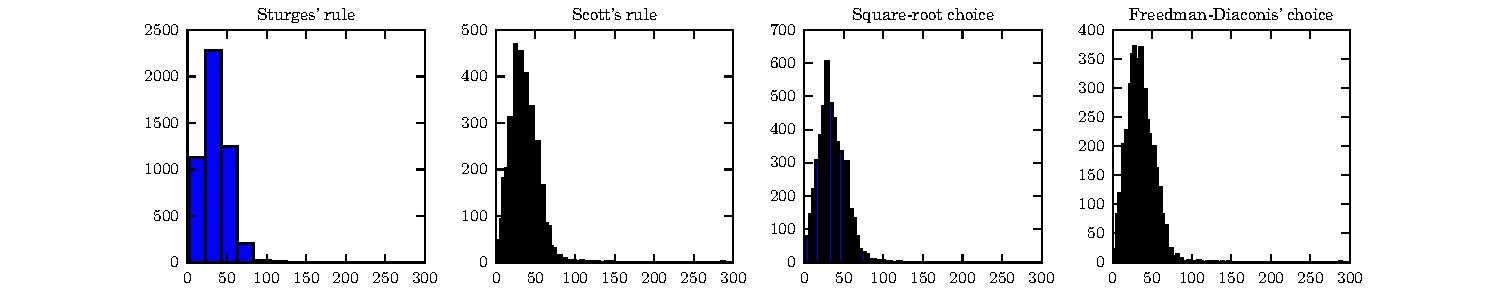
\includegraphics[width=\textwidth]{histograms/free_sulfur_dioxide.pdf}
\caption{Histograms of attribute \emph{free sulfur dioxide} using different binning methods}\end{figure}

\begin{figure}[H]
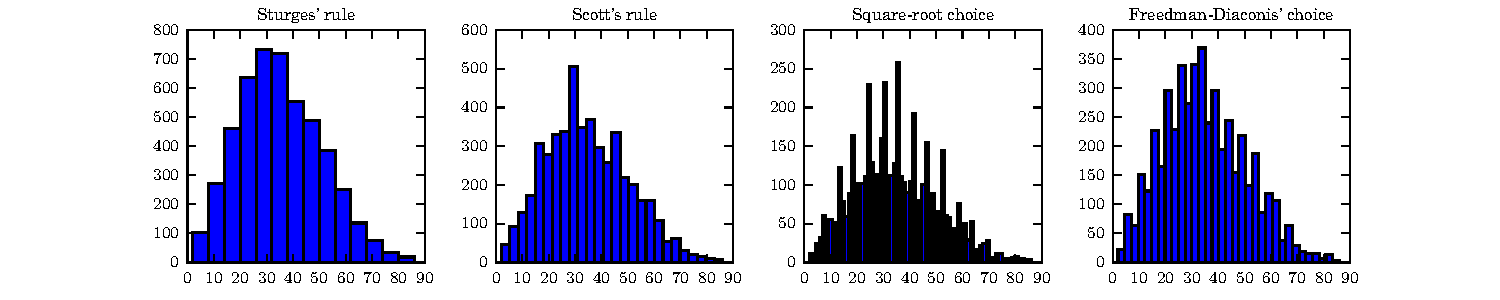
\includegraphics[width=\textwidth]{histograms/free_sulfur_dioxide_filtered.pdf}
\caption{Histograms of attribute \emph{free sulfur dioxide} with outliers further than 3 standard deviations from the mean filtered}
\end{figure}

\begin{figure}[H]
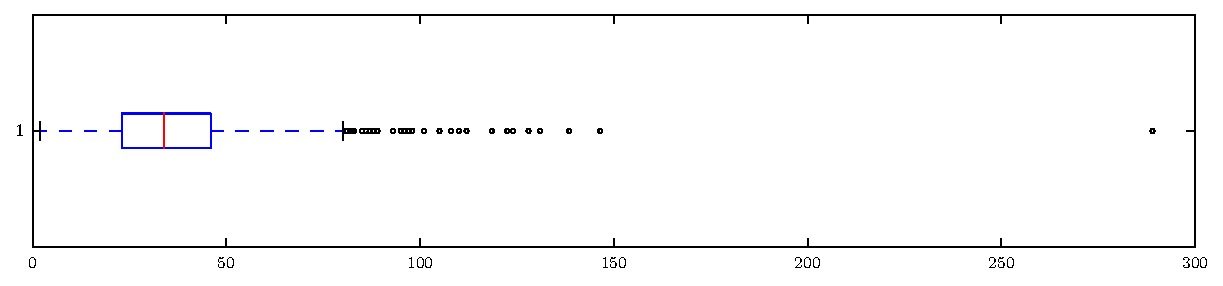
\includegraphics[width=\textwidth]{boxplots/free_sulfur_dioxide.pdf}
\caption{Boxplot of attribute \emph{free sulfur dioxide}. Outside the one outlier near value 300, the values are near the mean.}\end{figure}

\newpage
\subsection{total sulfur dioxide}
\begin{figure}[H]
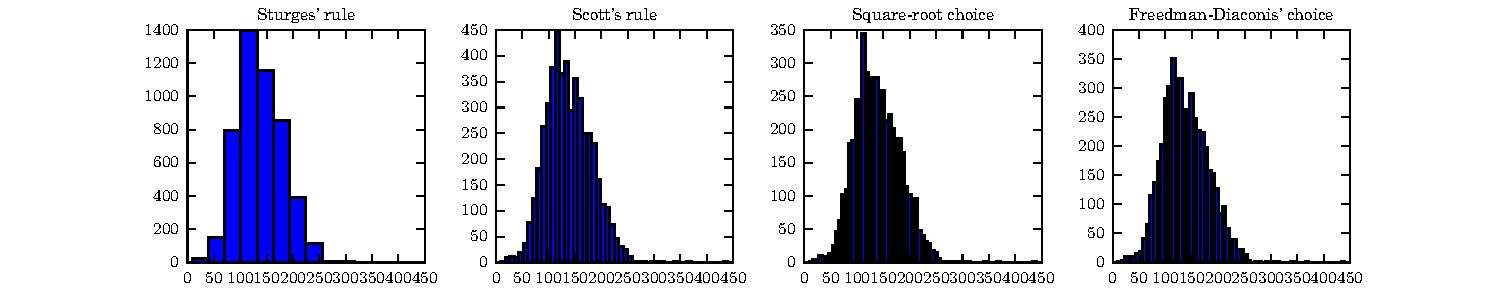
\includegraphics[width=\textwidth]{histograms/total_sulfur_dioxide.pdf}
\caption{Histograms of attribute \emph{total sulfur dioxide} using different binning methods}\end{figure}

\begin{figure}[H]
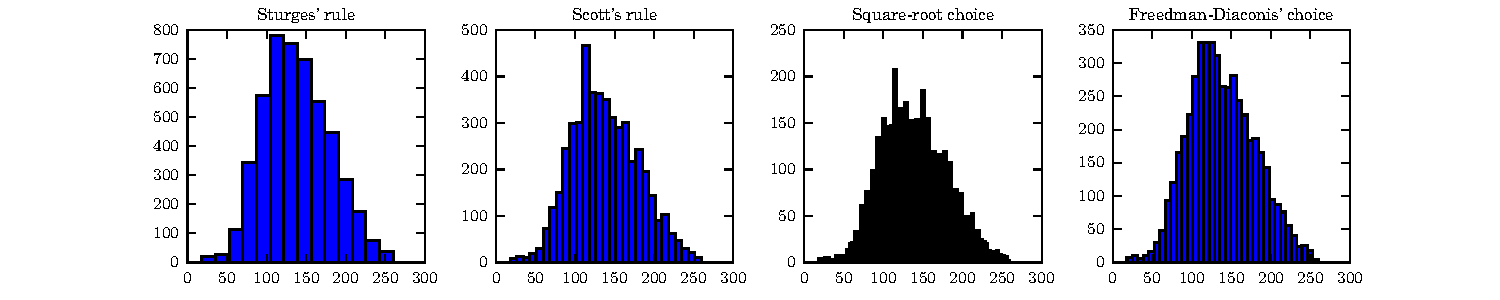
\includegraphics[width=\textwidth]{histograms/total_sulfur_dioxide_filtered.pdf}
\caption{Histograms of attribute \emph{total sulfur dioxide} with outliers further than 3 standard deviations from the mean filtered}
\end{figure}

\begin{figure}[H]
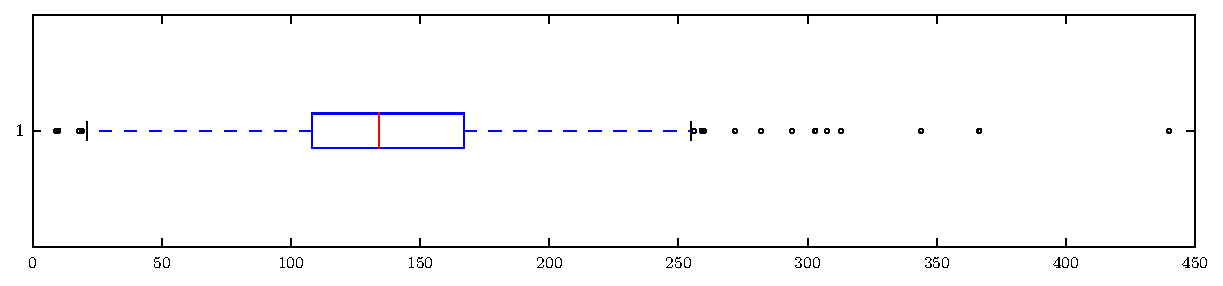
\includegraphics[width=\textwidth]{boxplots/total_sulfur_dioxide.pdf}
\caption{Boxplot of attribute \emph{total sulfur dioxide}. The values are quite spread out, and there are a few outliers.}\end{figure}

\newpage
\subsection{alcohol}
\begin{figure}[H]
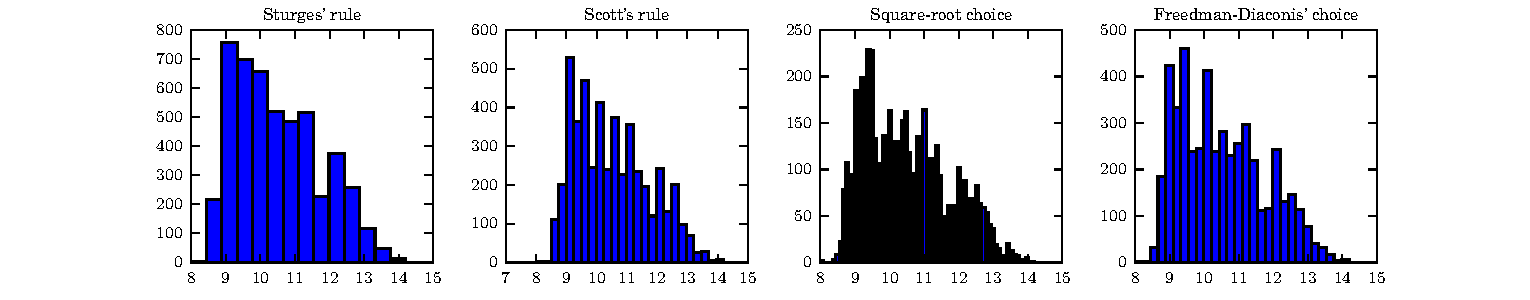
\includegraphics[width=\textwidth]{histograms/alcohol.pdf}
\caption{Histograms of attribute \emph{alcohol} using different binning methods}\end{figure}

\begin{figure}[H]
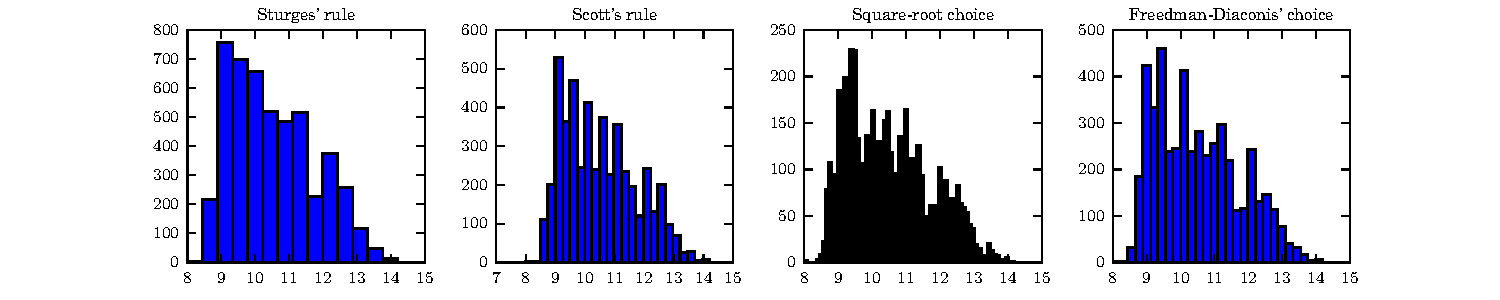
\includegraphics[width=\textwidth]{histograms/alcohol_filtered.pdf}
\caption{Histograms of attribute \emph{alcohol} with outliers further than 3 standard deviations from the mean filtered}
\end{figure}

\begin{figure}[H]
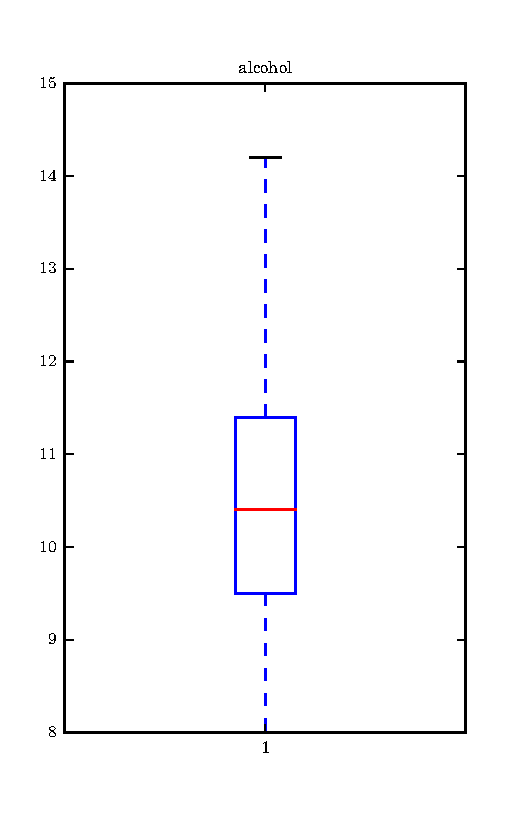
\includegraphics[width=\textwidth]{boxplots/alcohol.pdf}
\caption{Boxplot of attribute \emph{alcohol}. No outliers present, the values are in a really limited range.}\end{figure}

\newpage
\subsection{volatile acidity}
\begin{figure}[H]
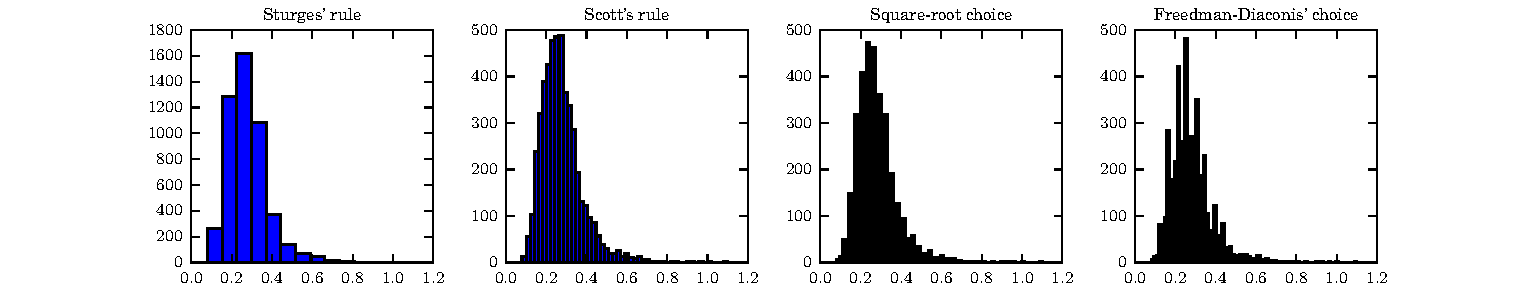
\includegraphics[width=\textwidth]{histograms/volatile_acidity.pdf}
\caption{Histograms of attribute \emph{volatile acidity} using different binning methods}\end{figure}

\begin{figure}[H]
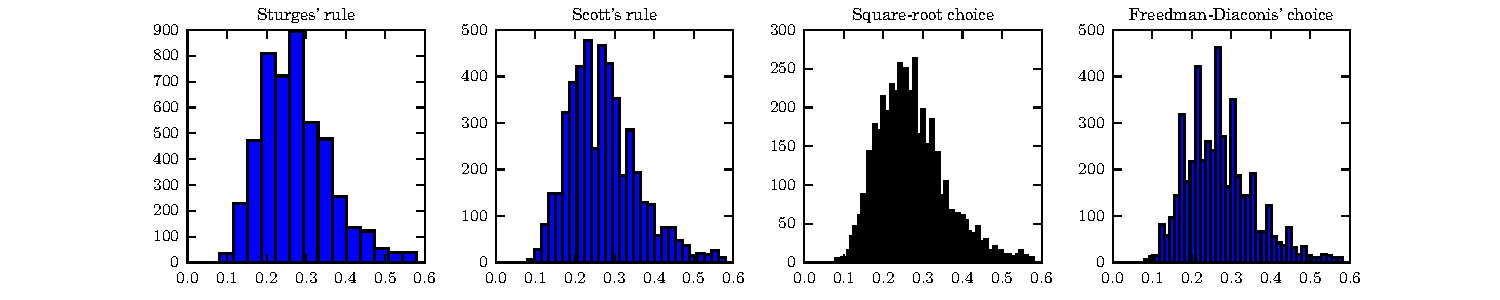
\includegraphics[width=\textwidth]{histograms/volatile_acidity_filtered.pdf}
\caption{Histograms of attribute \emph{volatile acidity} with outliers further than 3 standard deviations from the mean filtered}
\end{figure}

\begin{figure}[H]
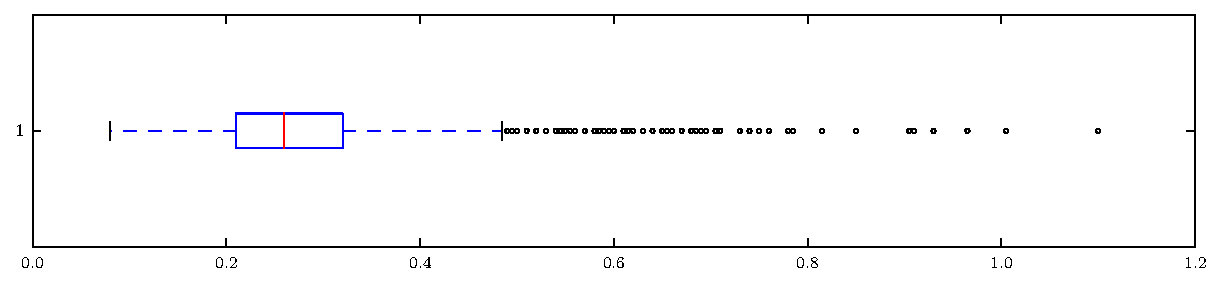
\includegraphics[width=\textwidth]{boxplots/volatile_acidity.pdf}
\caption{Boxplot of attribute \emph{volatile acidity}. Like in \emph{free sulfur dioxide}, the upper end of the value set is quite spread out.}\end{figure}

\newpage
\subsection{sulphates}
\begin{figure}[H]
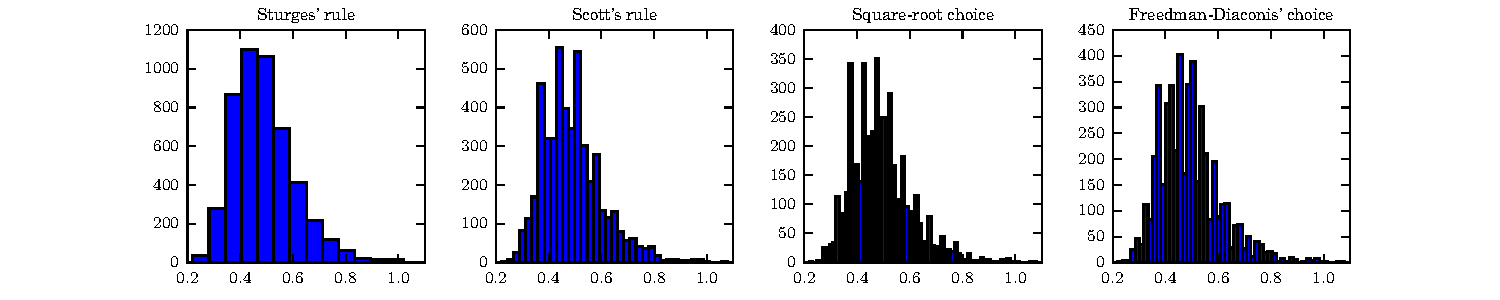
\includegraphics[width=\textwidth]{histograms/sulphates.pdf}
\caption{Histograms of attribute \emph{sulphates} using different binning methods}\end{figure}

\begin{figure}[H]
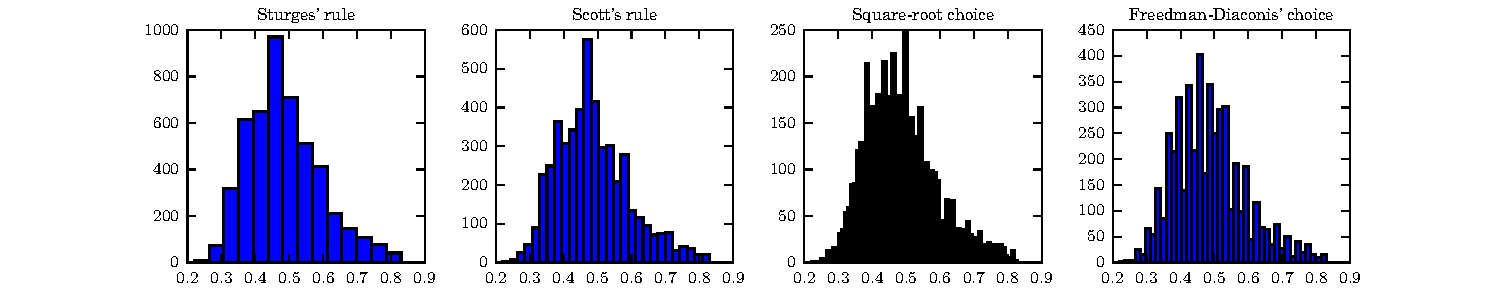
\includegraphics[width=\textwidth]{histograms/sulphates_filtered.pdf}
\caption{Histograms of attribute \emph{sulphates} with outliers further than 3 standard deviations from the mean filtered}
\end{figure}

\begin{figure}[H]
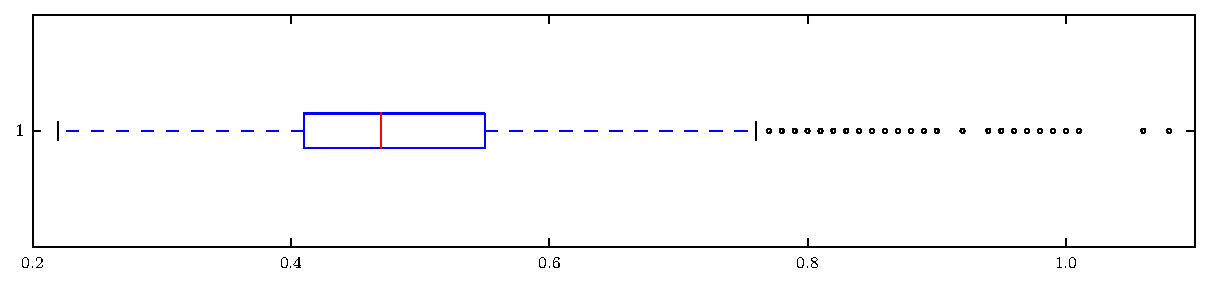
\includegraphics[width=\textwidth]{boxplots/sulphates.pdf}
\caption{Boxplot of attribute \emph{sulphates}. Like in \emph{free sulfur dioxide}, the upper end of the value set is quite spread out.}\end{figure}

\newpage
\subsection{residual sugar}
\begin{figure}[H]
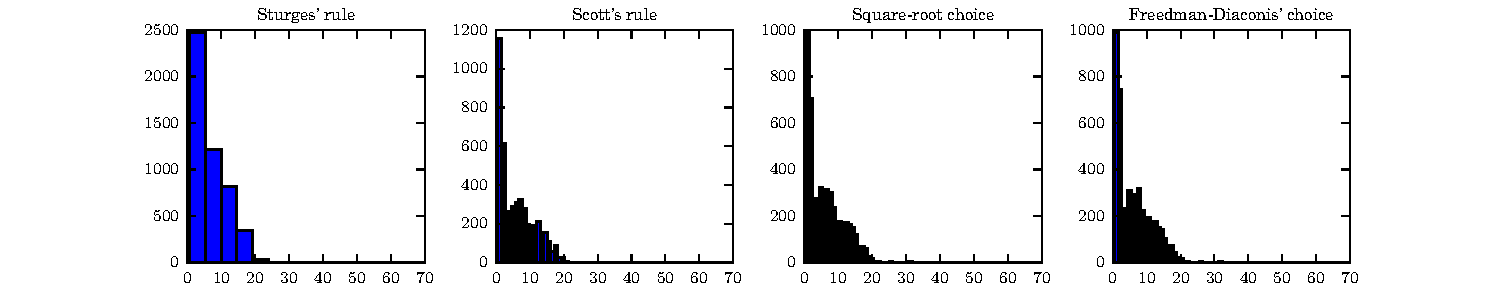
\includegraphics[width=\textwidth]{histograms/residual_sugar.pdf}
\caption{Histograms of attribute \emph{residual sugar} using different binning methods}\end{figure}

\begin{figure}[H]
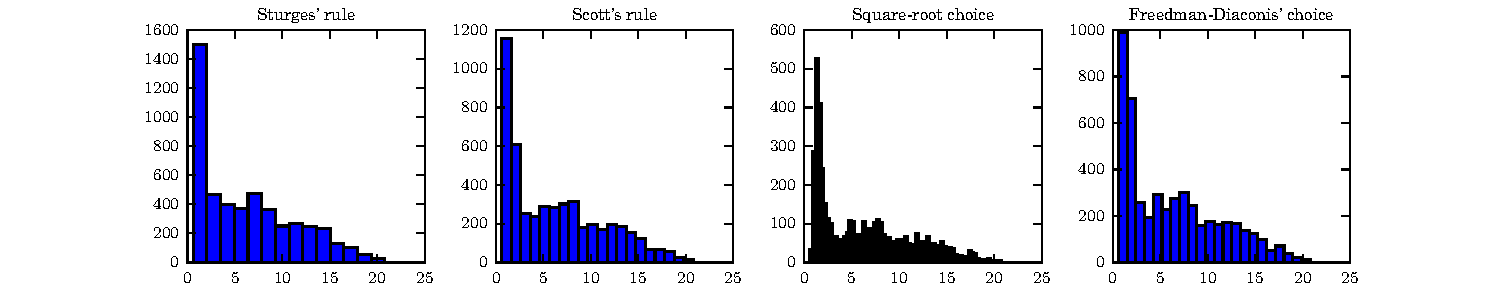
\includegraphics[width=\textwidth]{histograms/residual_sugar_filtered.pdf}
\caption{Histograms of attribute \emph{residual sugar} with outliers further than 3 standard deviations from the mean filtered}
\end{figure}

\begin{figure}[H]
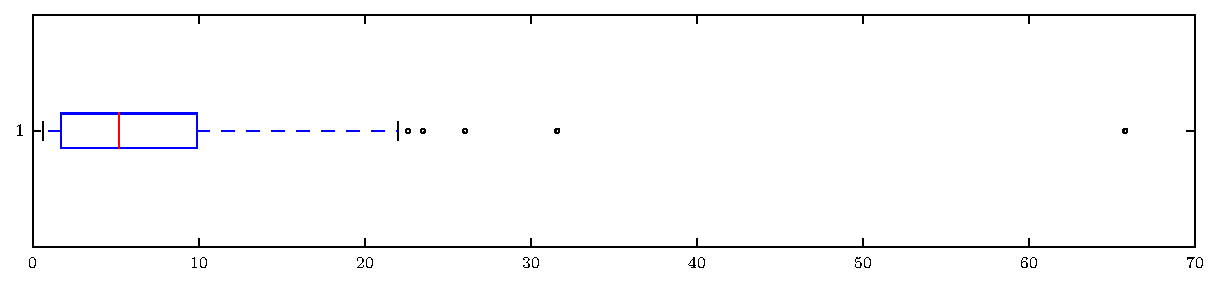
\includegraphics[width=\textwidth]{boxplots/residual_sugar.pdf}
\caption{Boxplot of attribute \emph{residual sugar}. There are a few outliers, but the values are otherwise really bunched together.}\end{figure}

\newpage
\subsection{pH}
\begin{figure}[H]
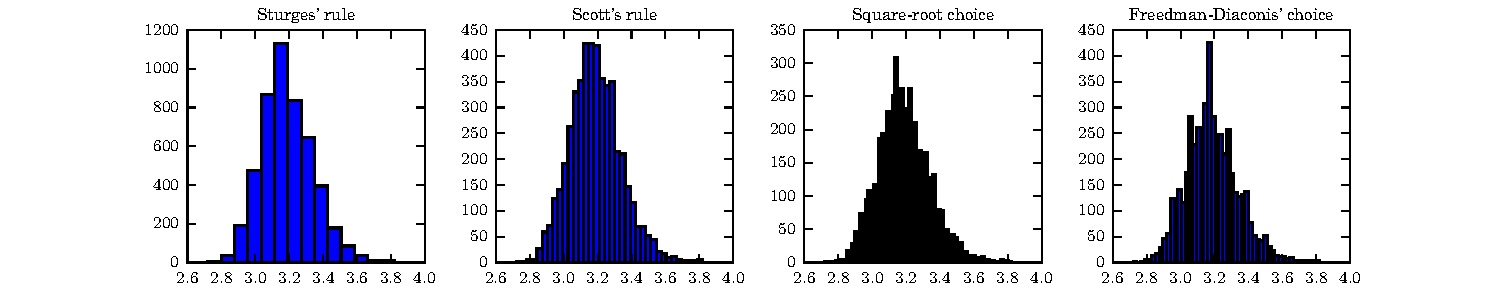
\includegraphics[width=\textwidth]{histograms/pH.pdf}
\caption{Histograms of attribute \emph{pH} using different binning methods}\end{figure}

\begin{figure}[H]
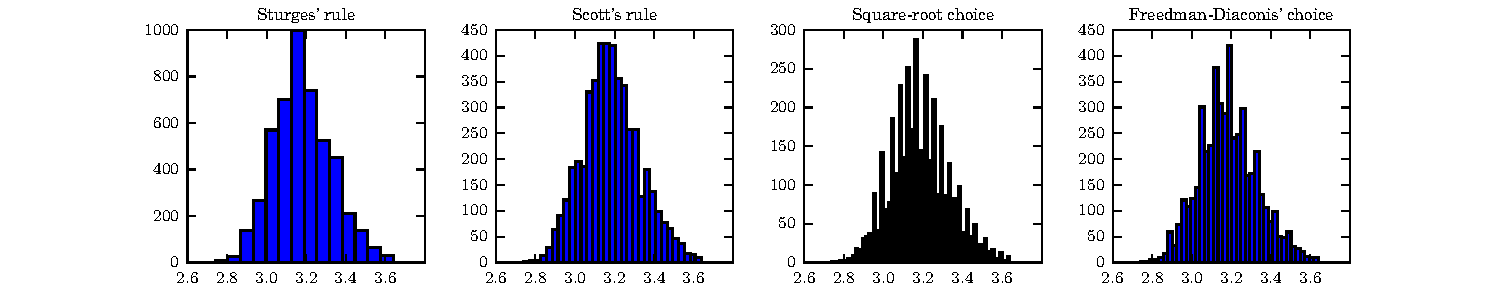
\includegraphics[width=\textwidth]{histograms/pH_filtered.pdf}
\caption{Histograms of attribute \emph{pH} with outliers further than 3 standard deviations from the mean filtered}
\end{figure}

\begin{figure}[H]
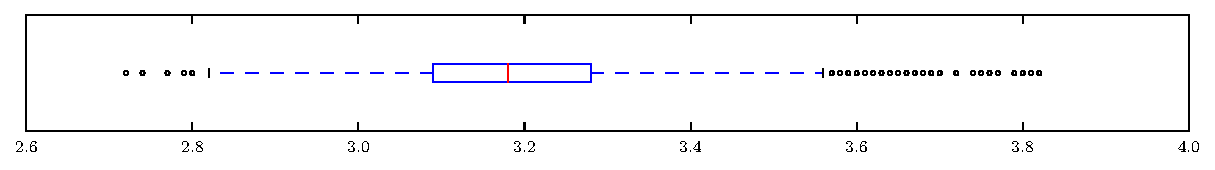
\includegraphics[width=\textwidth]{boxplots/pH.pdf}
\caption{Boxplot of attribute \emph{pH}. No distant outliers, the upper end of the range is once again more spread out.}\end{figure}

\newpage
\subsection{fixed acidity}
\begin{figure}[H]
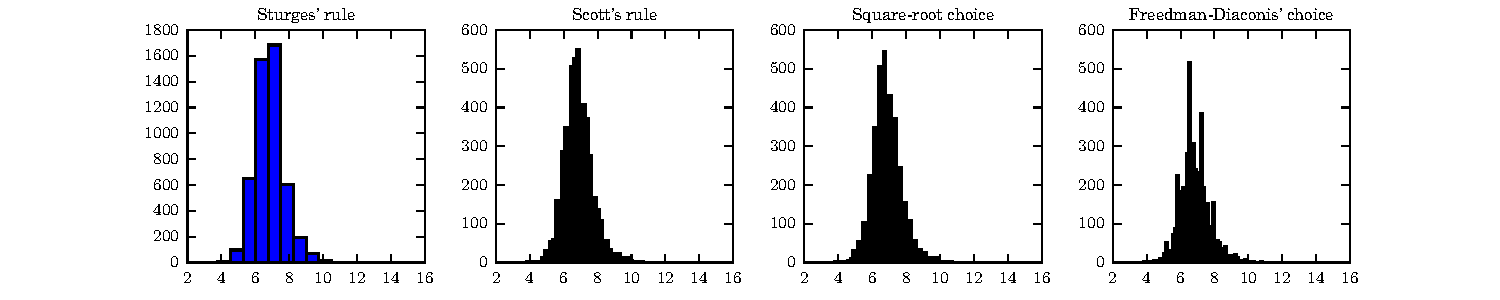
\includegraphics[width=\textwidth]{histograms/fixed_acidity.pdf}
\caption{Histograms of attribute \emph{fixed acidity} using different binning methods}\end{figure}

\begin{figure}[H]
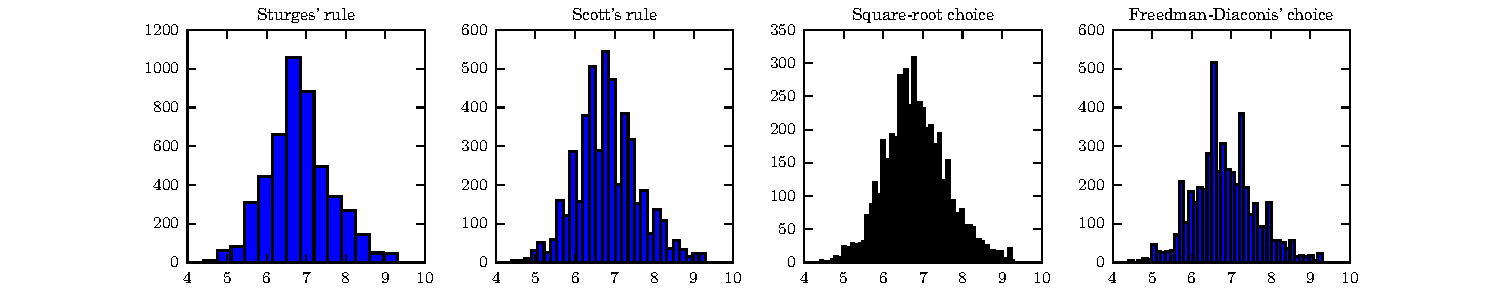
\includegraphics[width=\textwidth]{histograms/fixed_acidity_filtered.pdf}
\caption{Histograms of attribute \emph{fixed acidity} with outliers further than 3 standard deviations from the mean filtered}
\end{figure}

\begin{figure}[H]
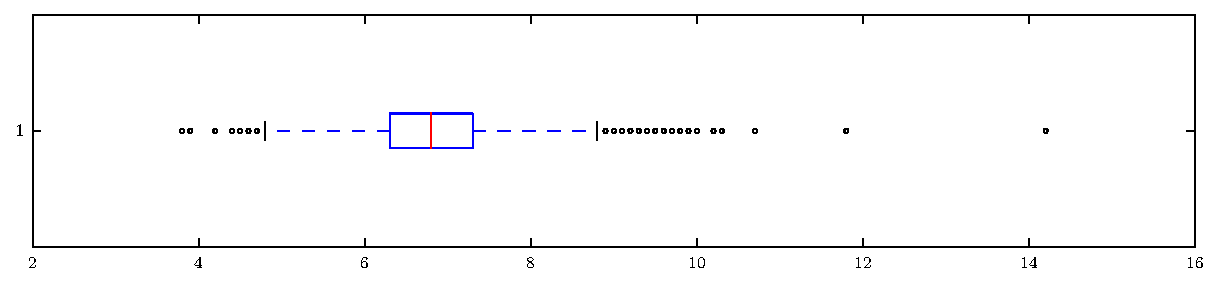
\includegraphics[width=\textwidth]{boxplots/fixed_acidity.pdf}
\caption{Boxplot of attribute \emph{fixed acidity}. A couple of outliers.}\end{figure}

\newpage
\subsection{density}
\begin{figure}[H]
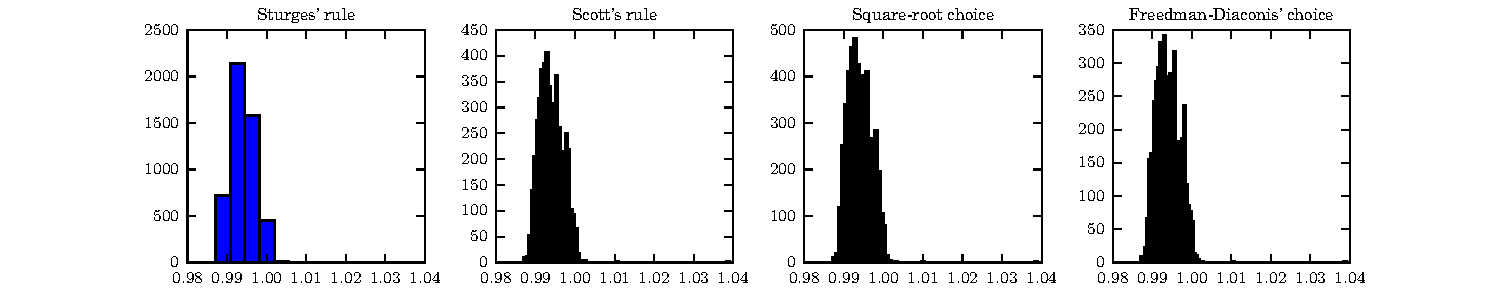
\includegraphics[width=\textwidth]{histograms/density.pdf}
\caption{Histograms of attribute \emph{density} using different binning methods}\end{figure}

\begin{figure}[H]
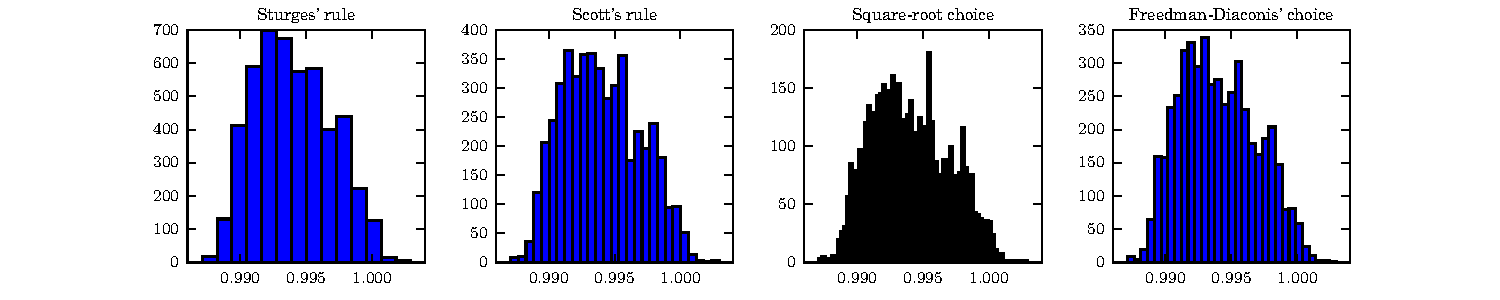
\includegraphics[width=\textwidth]{histograms/density_filtered.pdf}
\caption{Histograms of attribute \emph{density} with outliers further than 3 standard deviations from the mean filtered}
\end{figure}

\begin{figure}[H]
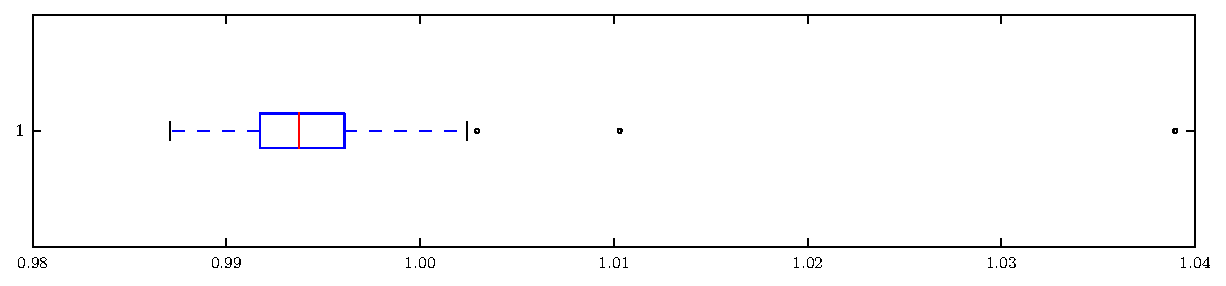
\includegraphics[width=\textwidth]{boxplots/density.pdf}
\caption{Boxplot of attribute \emph{density}. Some really distant outliers which could point at a measuring error.}\end{figure}

\newpage
\subsection{quality}
\begin{figure}[H]
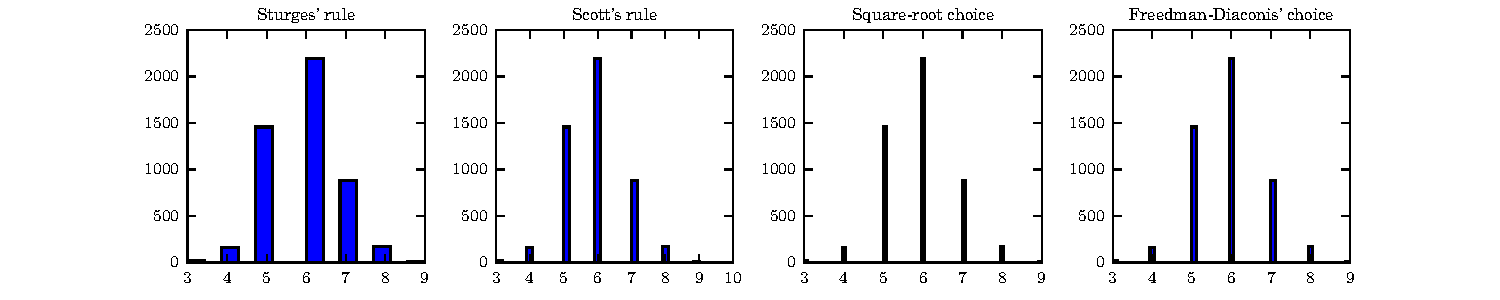
\includegraphics[width=\textwidth]{histograms/quality.pdf}
\caption{Histograms of attribute \emph{quality} using different binning methods}\end{figure}

\begin{figure}[H]
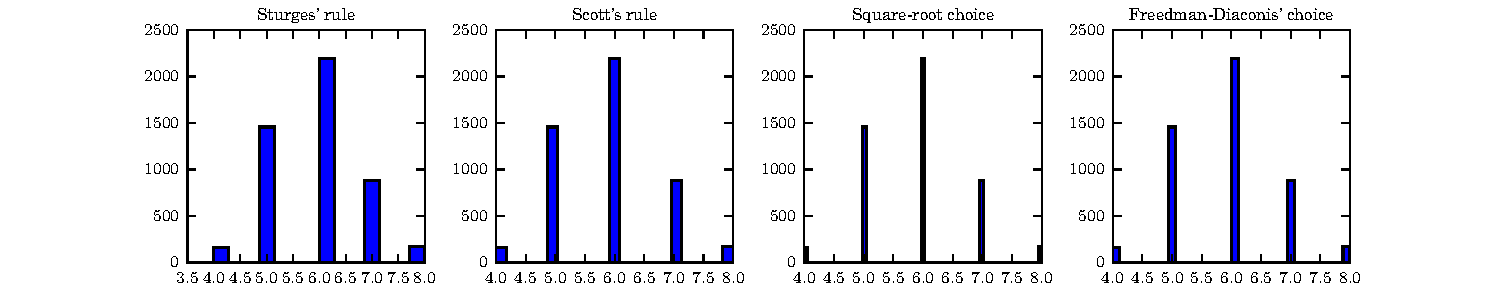
\includegraphics[width=\textwidth]{histograms/quality_filtered.pdf}
\caption{Histograms of attribute \emph{quality} with outliers further than 3 standard deviations from the mean filtered}
\end{figure}

\begin{figure}[H]
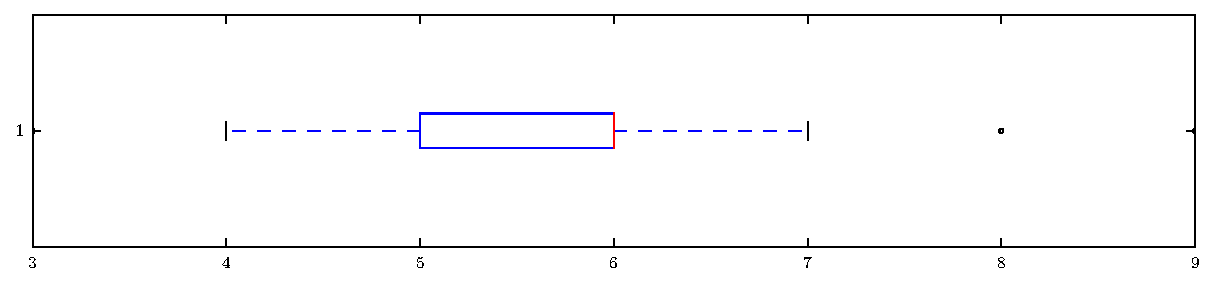
\includegraphics[width=\textwidth]{boxplots/quality.pdf}
\caption{Boxplot of attribute \emph{quality}. Due to the composition of the data set, all values of 3, 8 and 9 are treated as outliers.}\end{figure}

\newpage
\subsection{chlorides}
\begin{figure}[H]
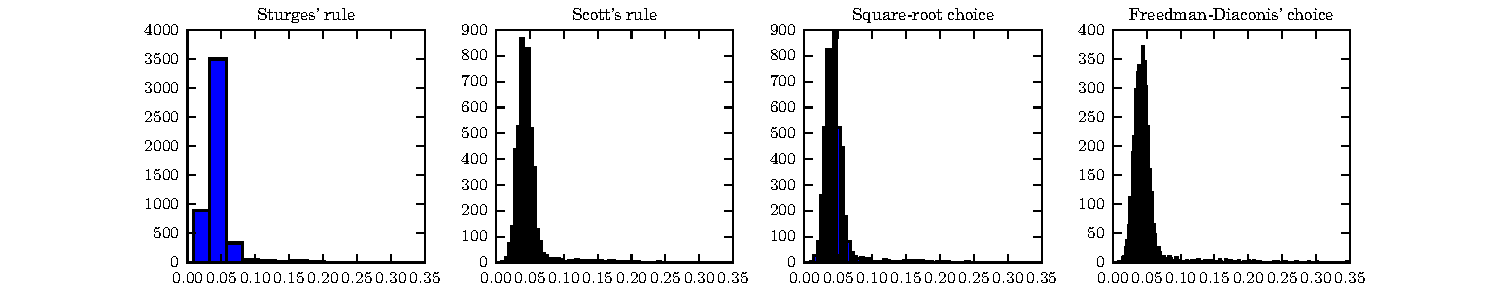
\includegraphics[width=\textwidth]{histograms/chlorides.pdf}
\caption{Histograms of attribute \emph{chlorides} using different binning methods}\end{figure}

\begin{figure}[H]
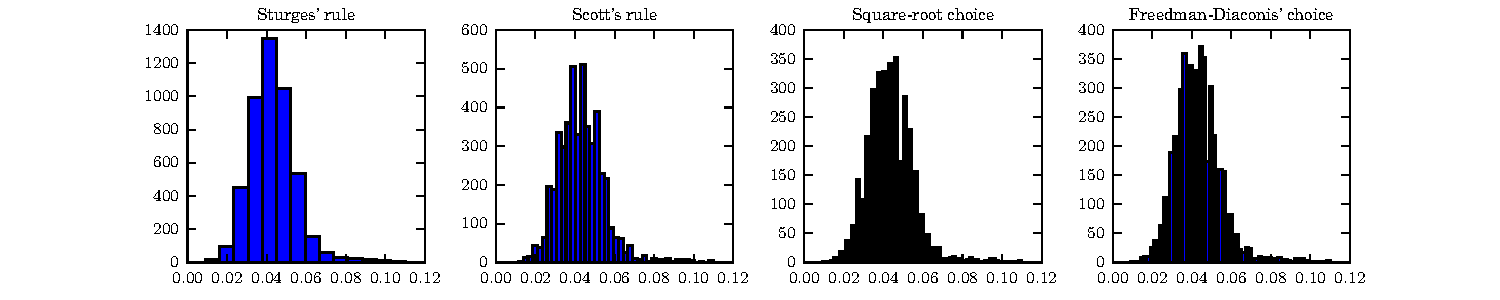
\includegraphics[width=\textwidth]{histograms/chlorides_filtered.pdf}
\caption{Histograms of attribute \emph{chlorides} with outliers further than 3 standard deviations from the mean filtered}
\end{figure}

\begin{figure}[H]
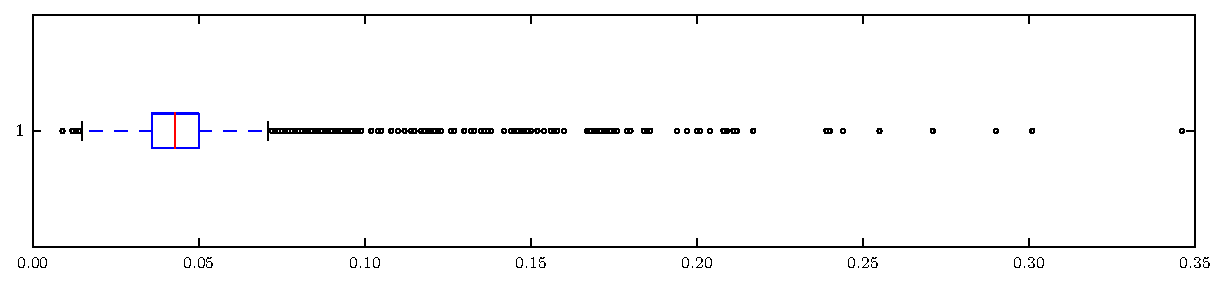
\includegraphics[width=\textwidth]{boxplots/chlorides.pdf}
\caption{Boxplot of attribute \emph{chlorides}. Really spread value set at the upper end of the spectrum.}\end{figure}

\newpage
\section{Plots for the whole feature set}
The scatter matrices were produced by making a $12\times 12$-subplot using \texttt{matplotlib}, writing out the feature titles to the diagonal and plotting the corresponding features against each other to all the remaining subplots. In case of the filtered version, the sets were first filtered to drop out all data points where one of the values used was further than 3 standard deviations from the mean.

The parallel coordinates representation was made using a $1\times 11$-subplot with all the ticks hidden by normalizing the data set to range (0...1), ordering the features by their correlation coefficients against the feature \textit{quality} and plotting all the feature pairs to the plots using the values of quality as the color. Due to the large number of data points, the unbalanced amounts of different qualities, and the relatively low correlation between multiple features, the resulting plot is quite obscure.

\begin{figure}[H]
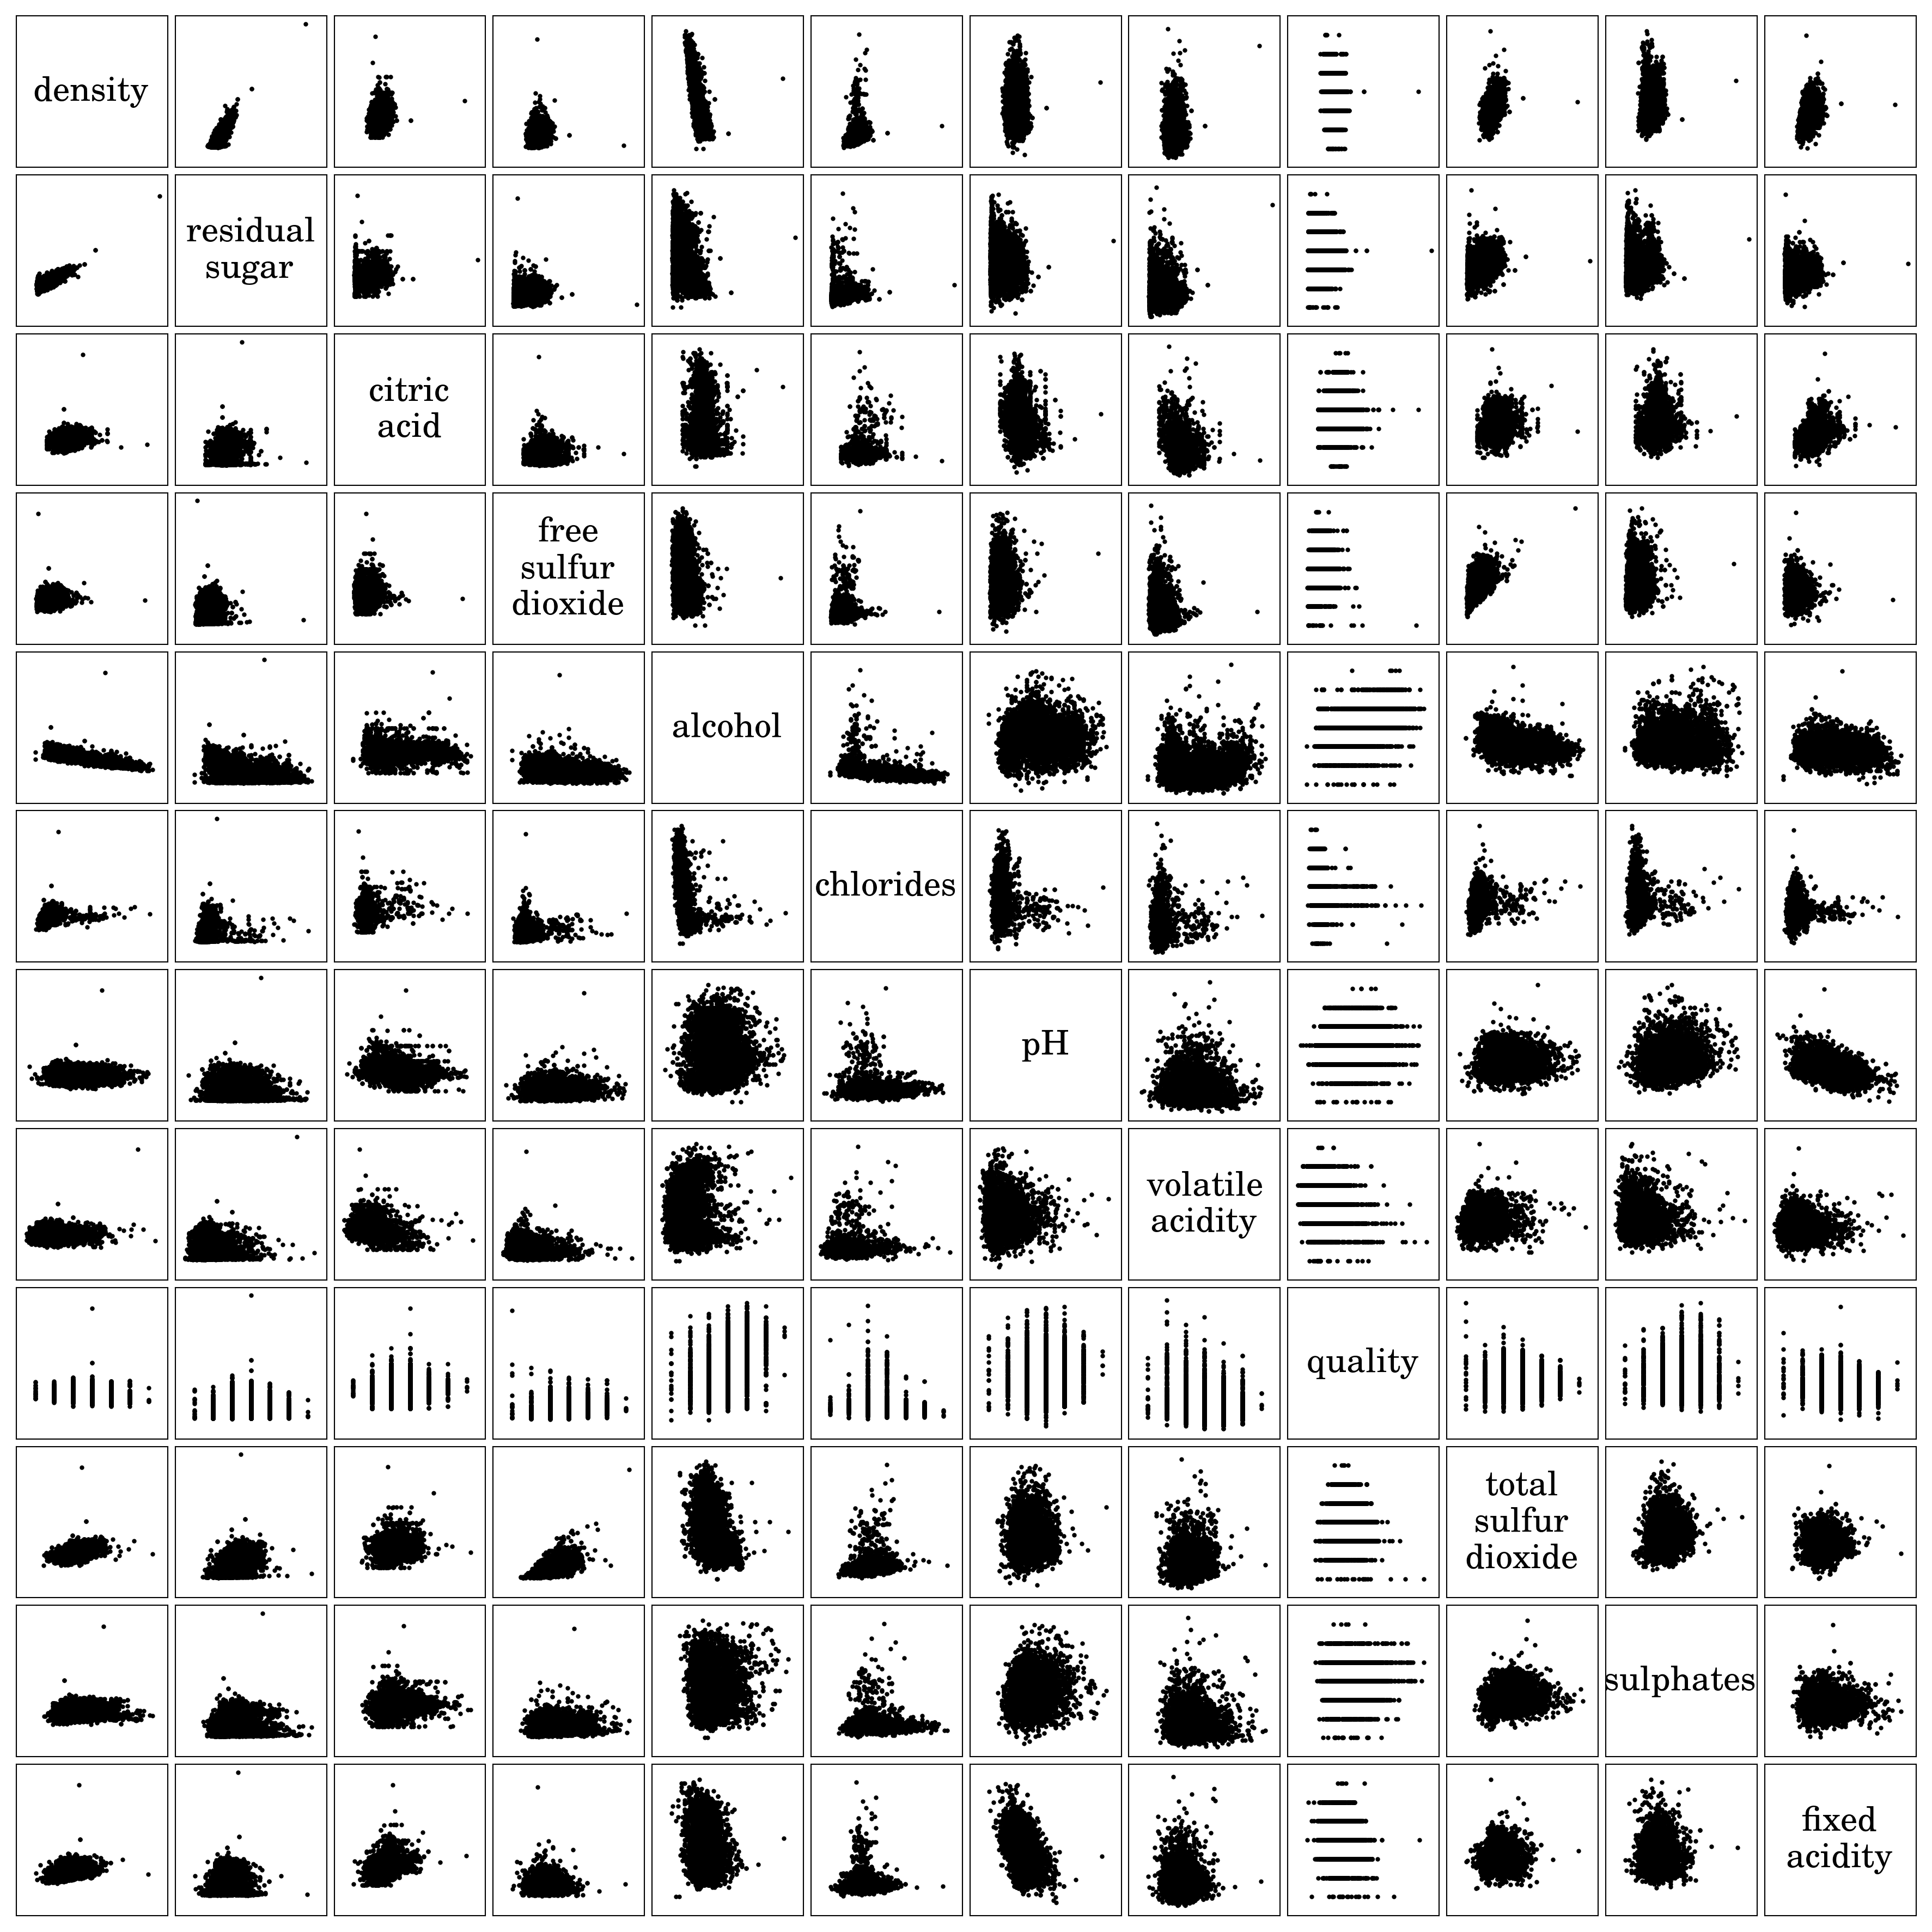
\includegraphics[width=\textwidth]{scattermatrix.png}
\caption{Scatter matrix of the whole feature set}
\end{figure}

\begin{figure}[H]
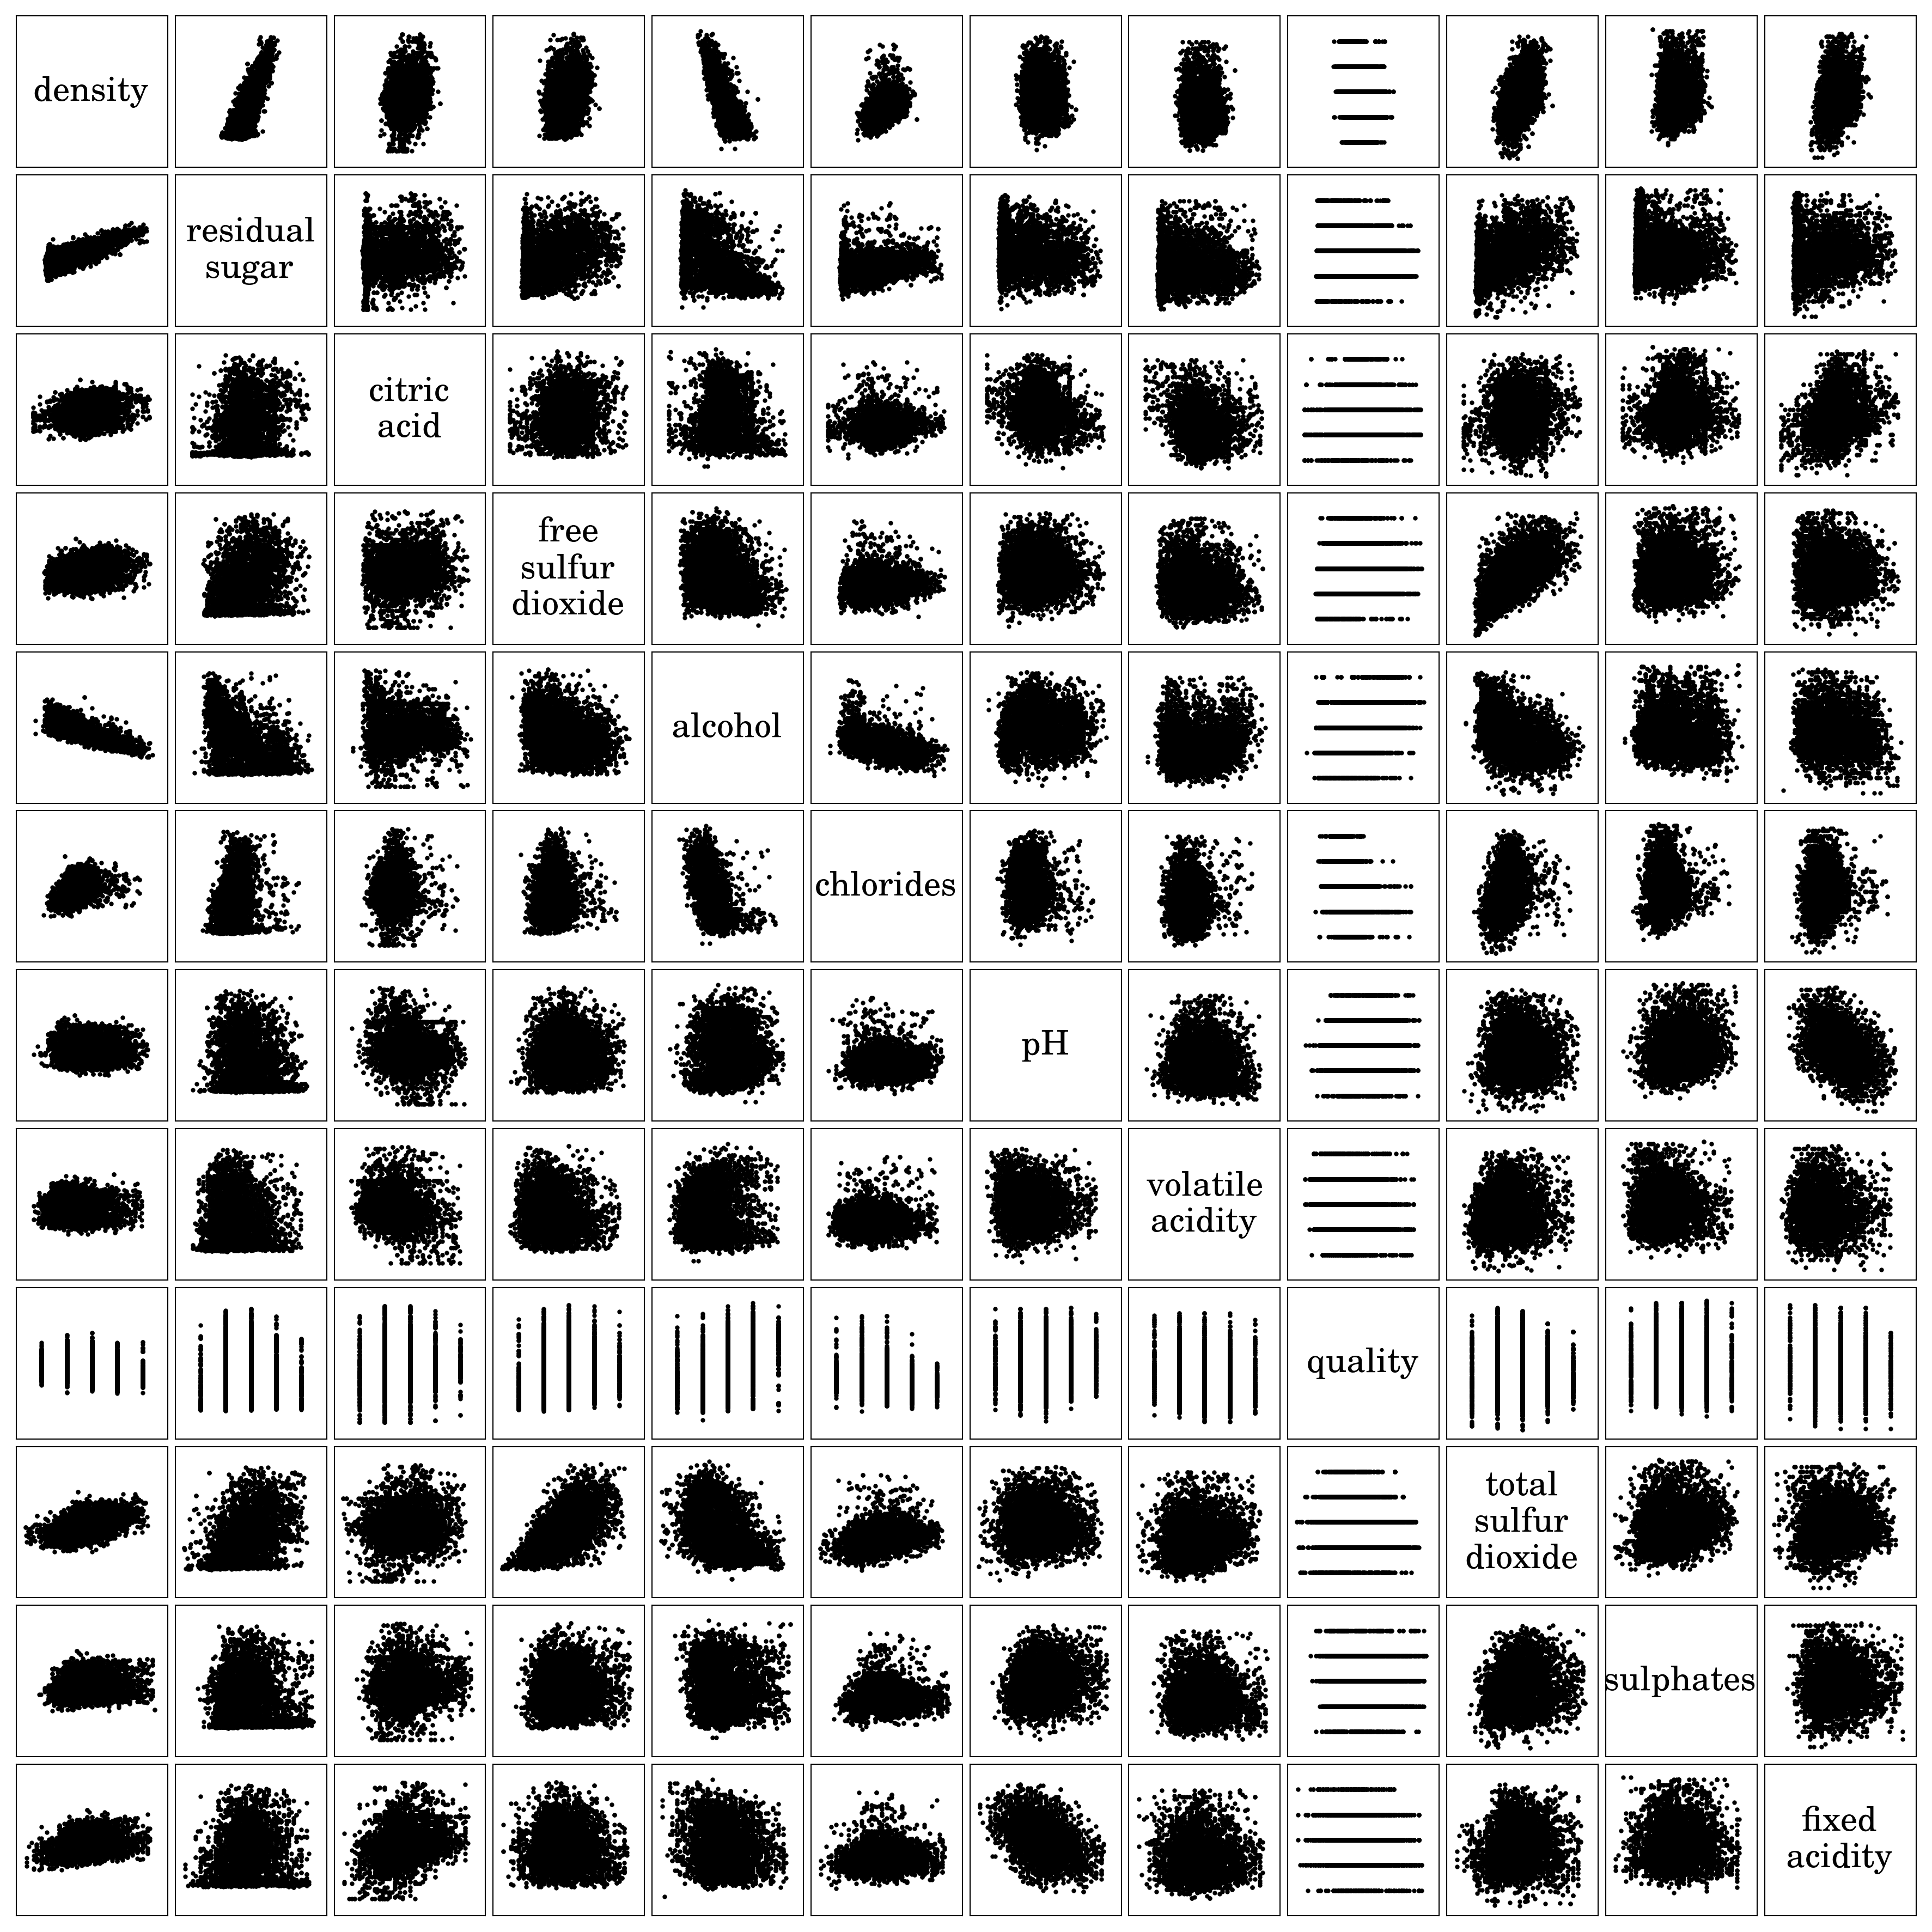
\includegraphics[width=\textwidth]{scattermatrix_filtered.png}
\caption{Scatter matrix of the whole feature set with outliers further than 3 standard deviations from the mean filtered}
\end{figure}

\begin{figure}[H]
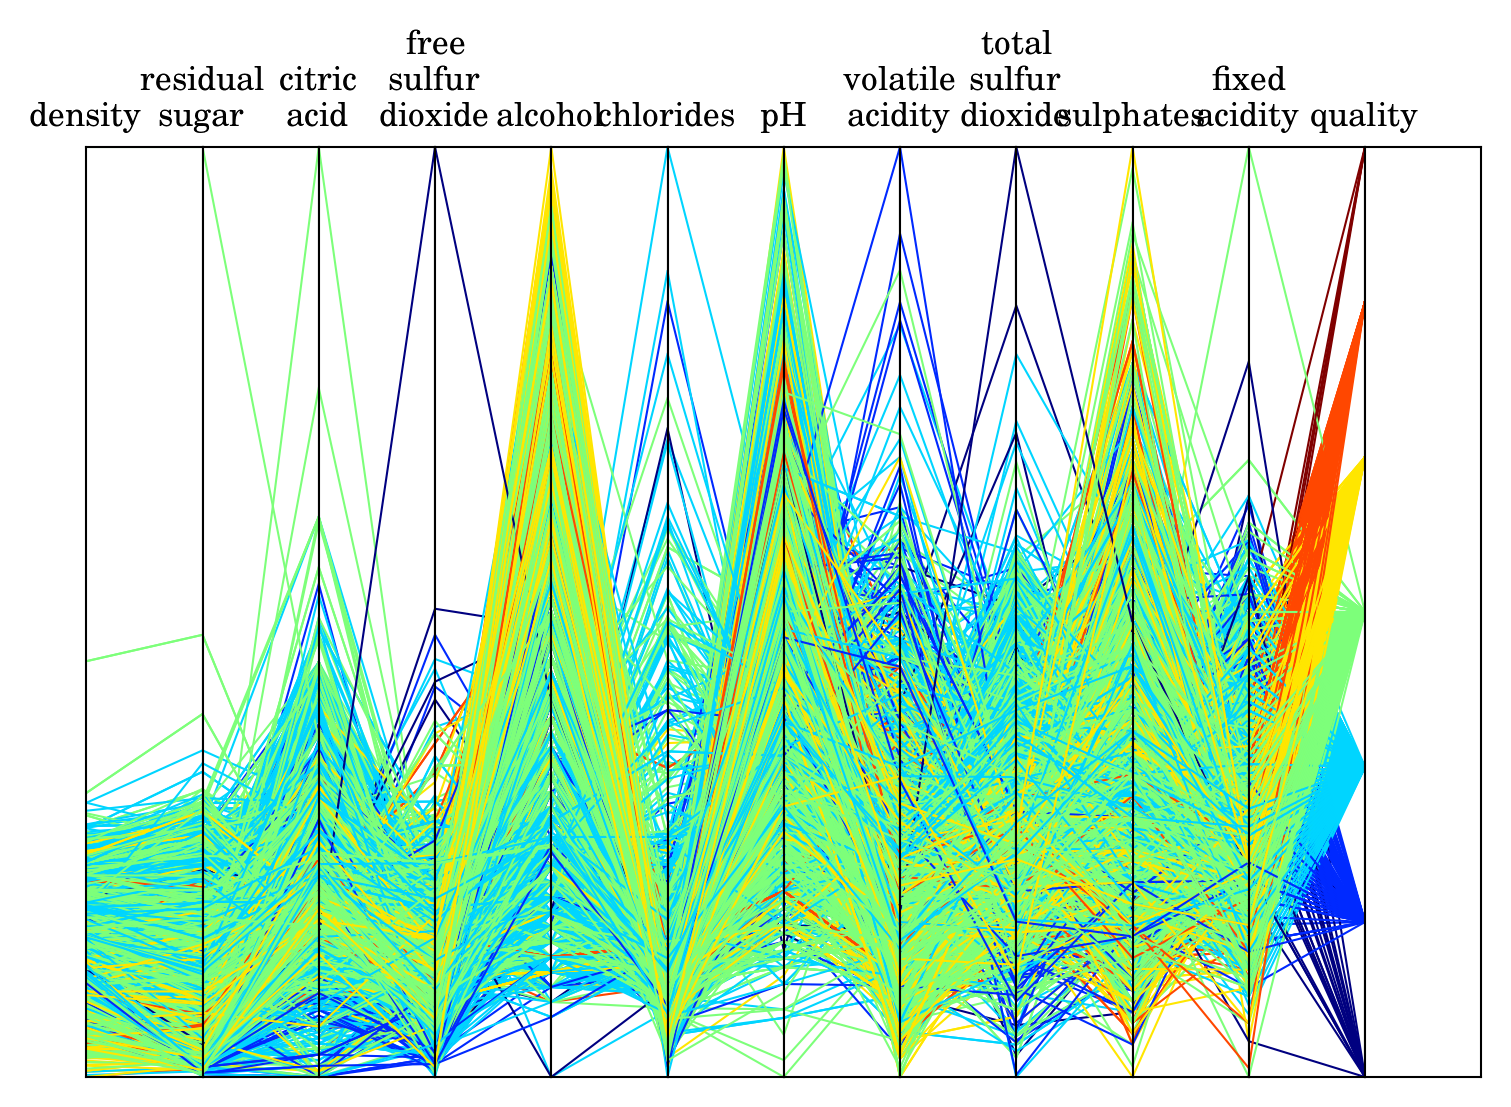
\includegraphics[width=\textwidth]{parallel_coords.png}
\caption{Parallel coordinates representation of the data set}
\end{figure}

\newpage
\section{Projections to 2D}
For the PCA representation the data was z-score standardized, then used to calculate a covariance matrix from which the eigenvectors and values were extracted. The resulting vector-value pairs were sorted based on the eigenvalues, and the first two vectors were turned into a $2\times 12$-matrix. This transformation matrix was multiplied with the standardized data matrix, and the resulting data was scatter plotted using the \textit{quality} values for coloring.

For MDS the data from aforementioned PCA was taken as the initial data, and using the multidimensional scaling algorithm the data was transformed using 25 iterations (which took nearly 2 hours) and $E_1$ as the objective function. The resulting data was plotted similarly to the PCA data.

\begin{table}[H]
\begin{adjustbox}{max width=\textwidth}
\begin{tabular}{l || *{13}{r}}
 & PC1 & PC2 & PC3 & PC4 & PC5 & PC6 & PC7 & PC8 & PC9 & PC10 & PC11 & PC12\\
\hline
Proportion of variance & 0.2746 & 0.1317 & 0.1170 & 0.0923 & 0.0856 & 0.0746 & 0.0654 & 0.0581 & 0.0469 & 0.0293 & 0.0226 & 0.0017\\
Cumulative variance &0.2746 & 0.4063 & 0.5234 & 0.6157 & 0.7013 & 0.7760 & 0.8414 & 0.8995 & 0.9464 & 0.9757 & 0.9983 & 1.0000\\
\end{tabular}
\end{adjustbox}
\caption{Singular and cumulative variances of the 12 principal components of the data}
\end{table}

The cumulative variance of principal components grows relatively slowly (9 out of 12 components required to get over 90\% of the variance preserved). This could imply that the correlation between features is low (as can be seen in \ref{ccs}), so they can not be presented with single vectors that easily. The 2D PCA projection in Figure \ref{pca} keeps only 40.63\% of the variance of the original data.

The results of multidimensional scaling shown in Figure \ref{mds} do not differ that much from PCA. There seems to be a clearer separation between lower and higher quality wines (implied using coloring, warmer colors are higher graded wines), but this could be caused by the drawing order of the points as well.

\begin{figure}[H]
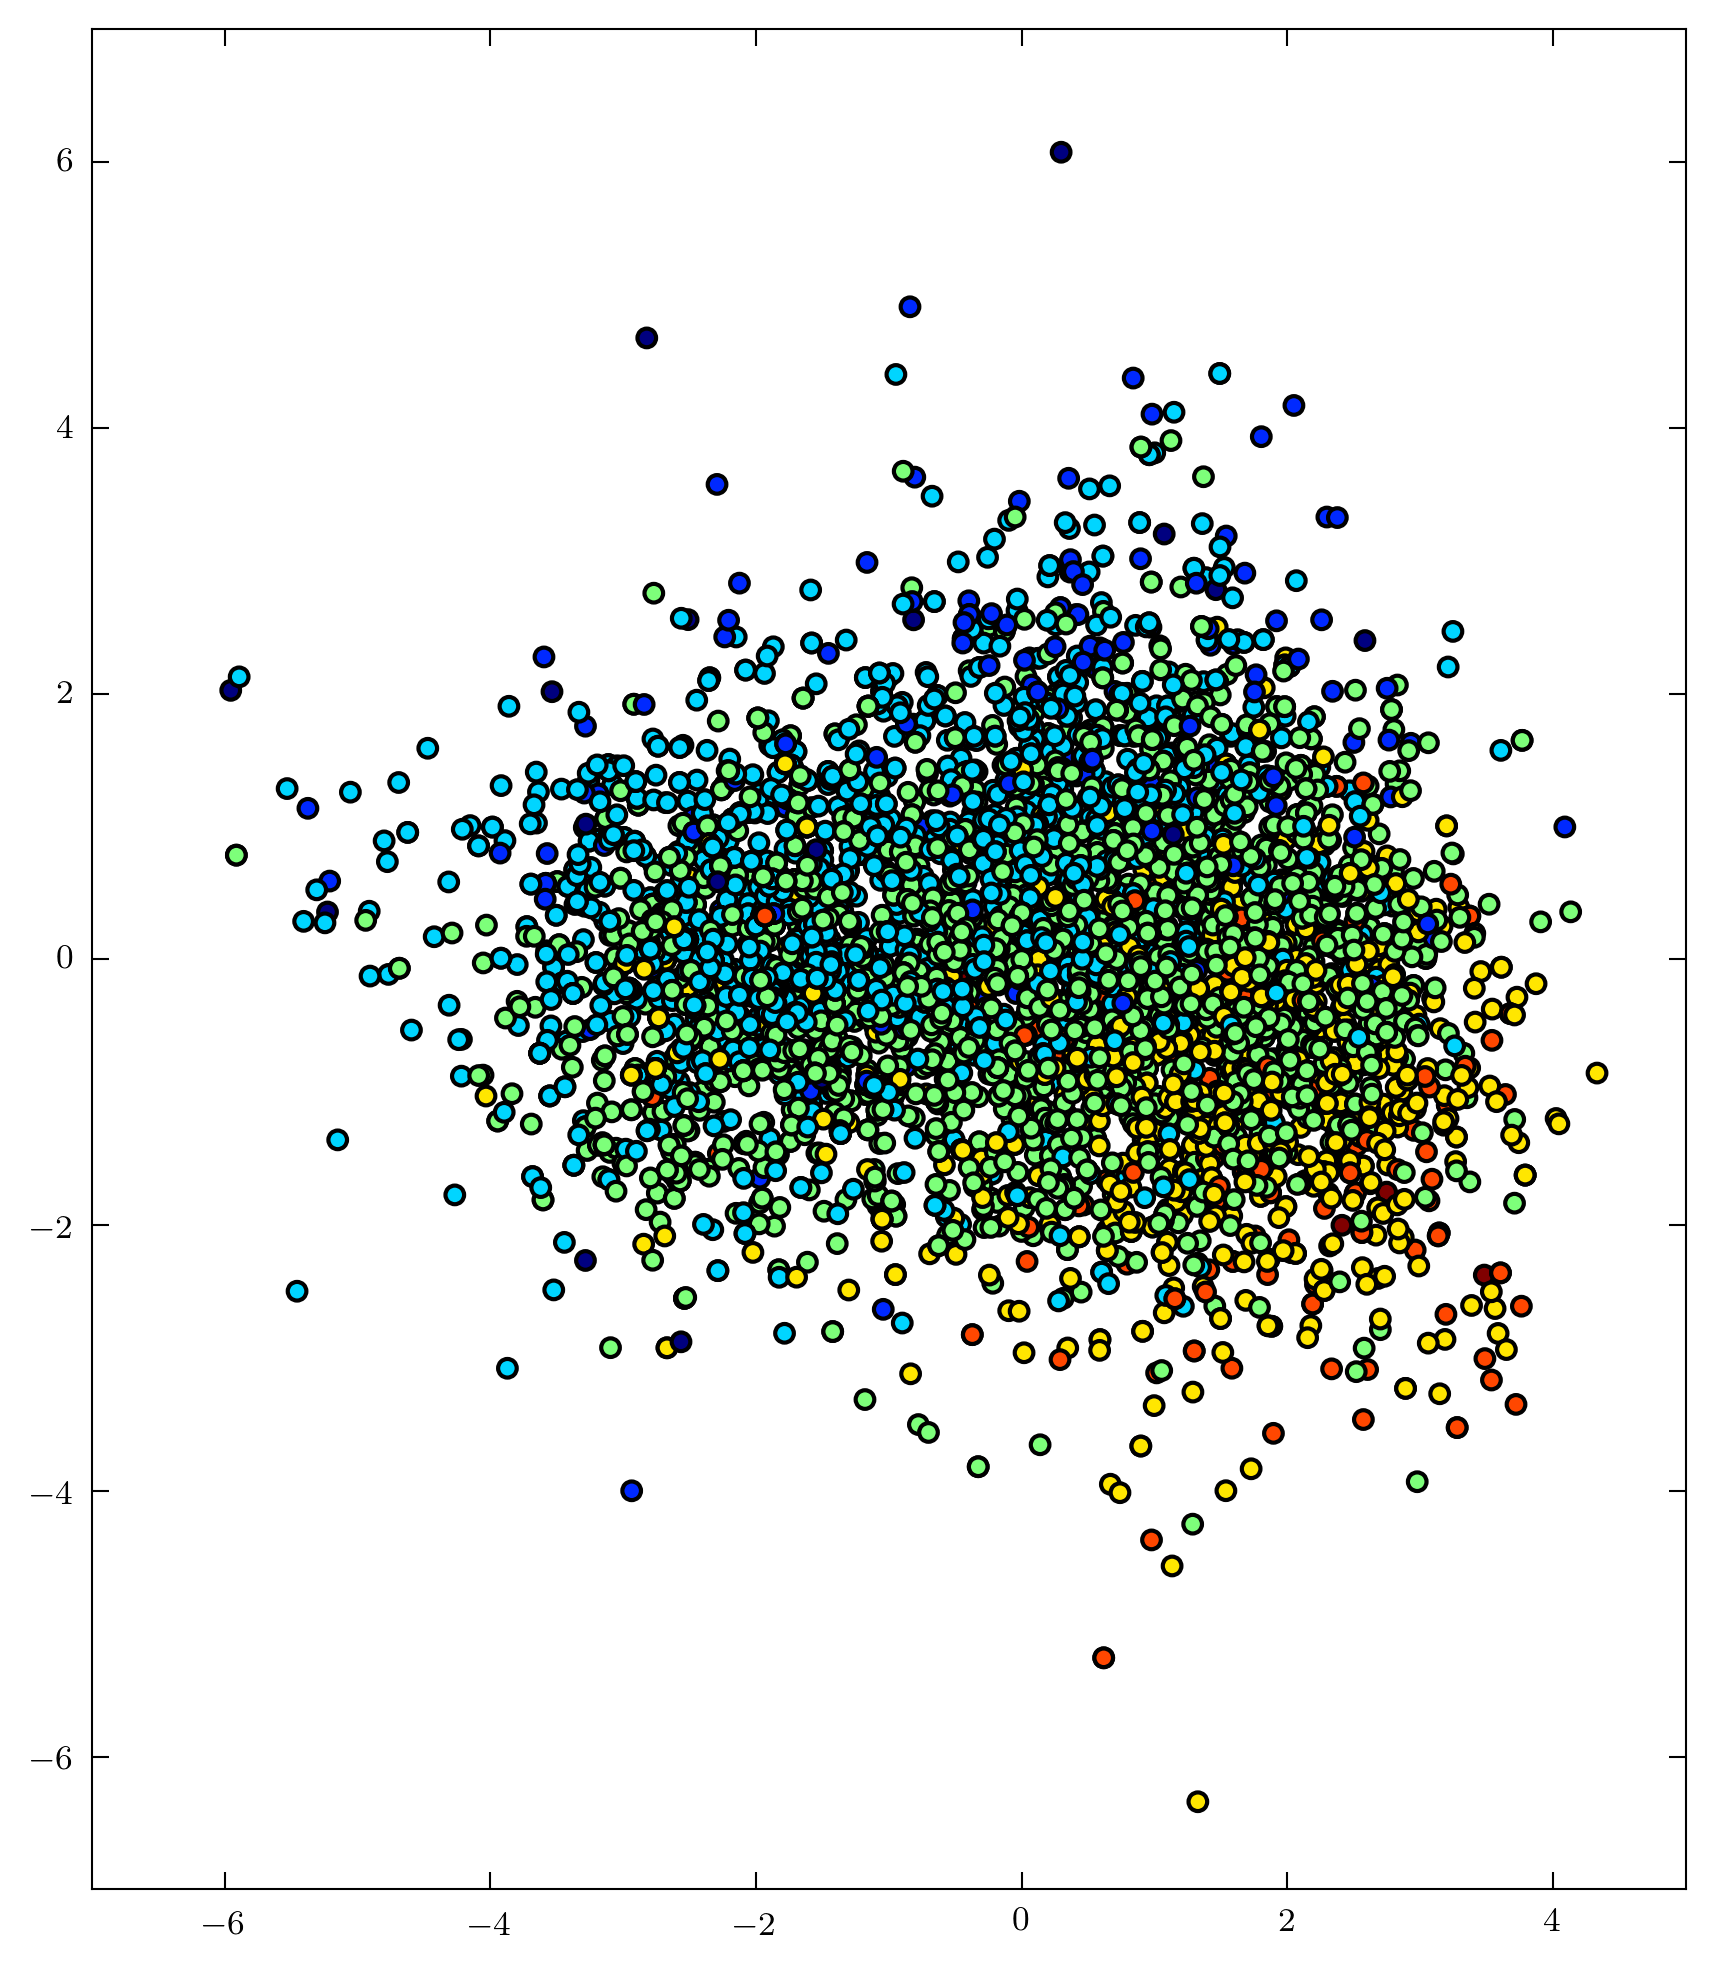
\includegraphics[width=\textwidth]{pca.png}
\caption{2D projection of the normalized data set using PCA}\end{figure}
\label{pca}
\begin{figure}[H]
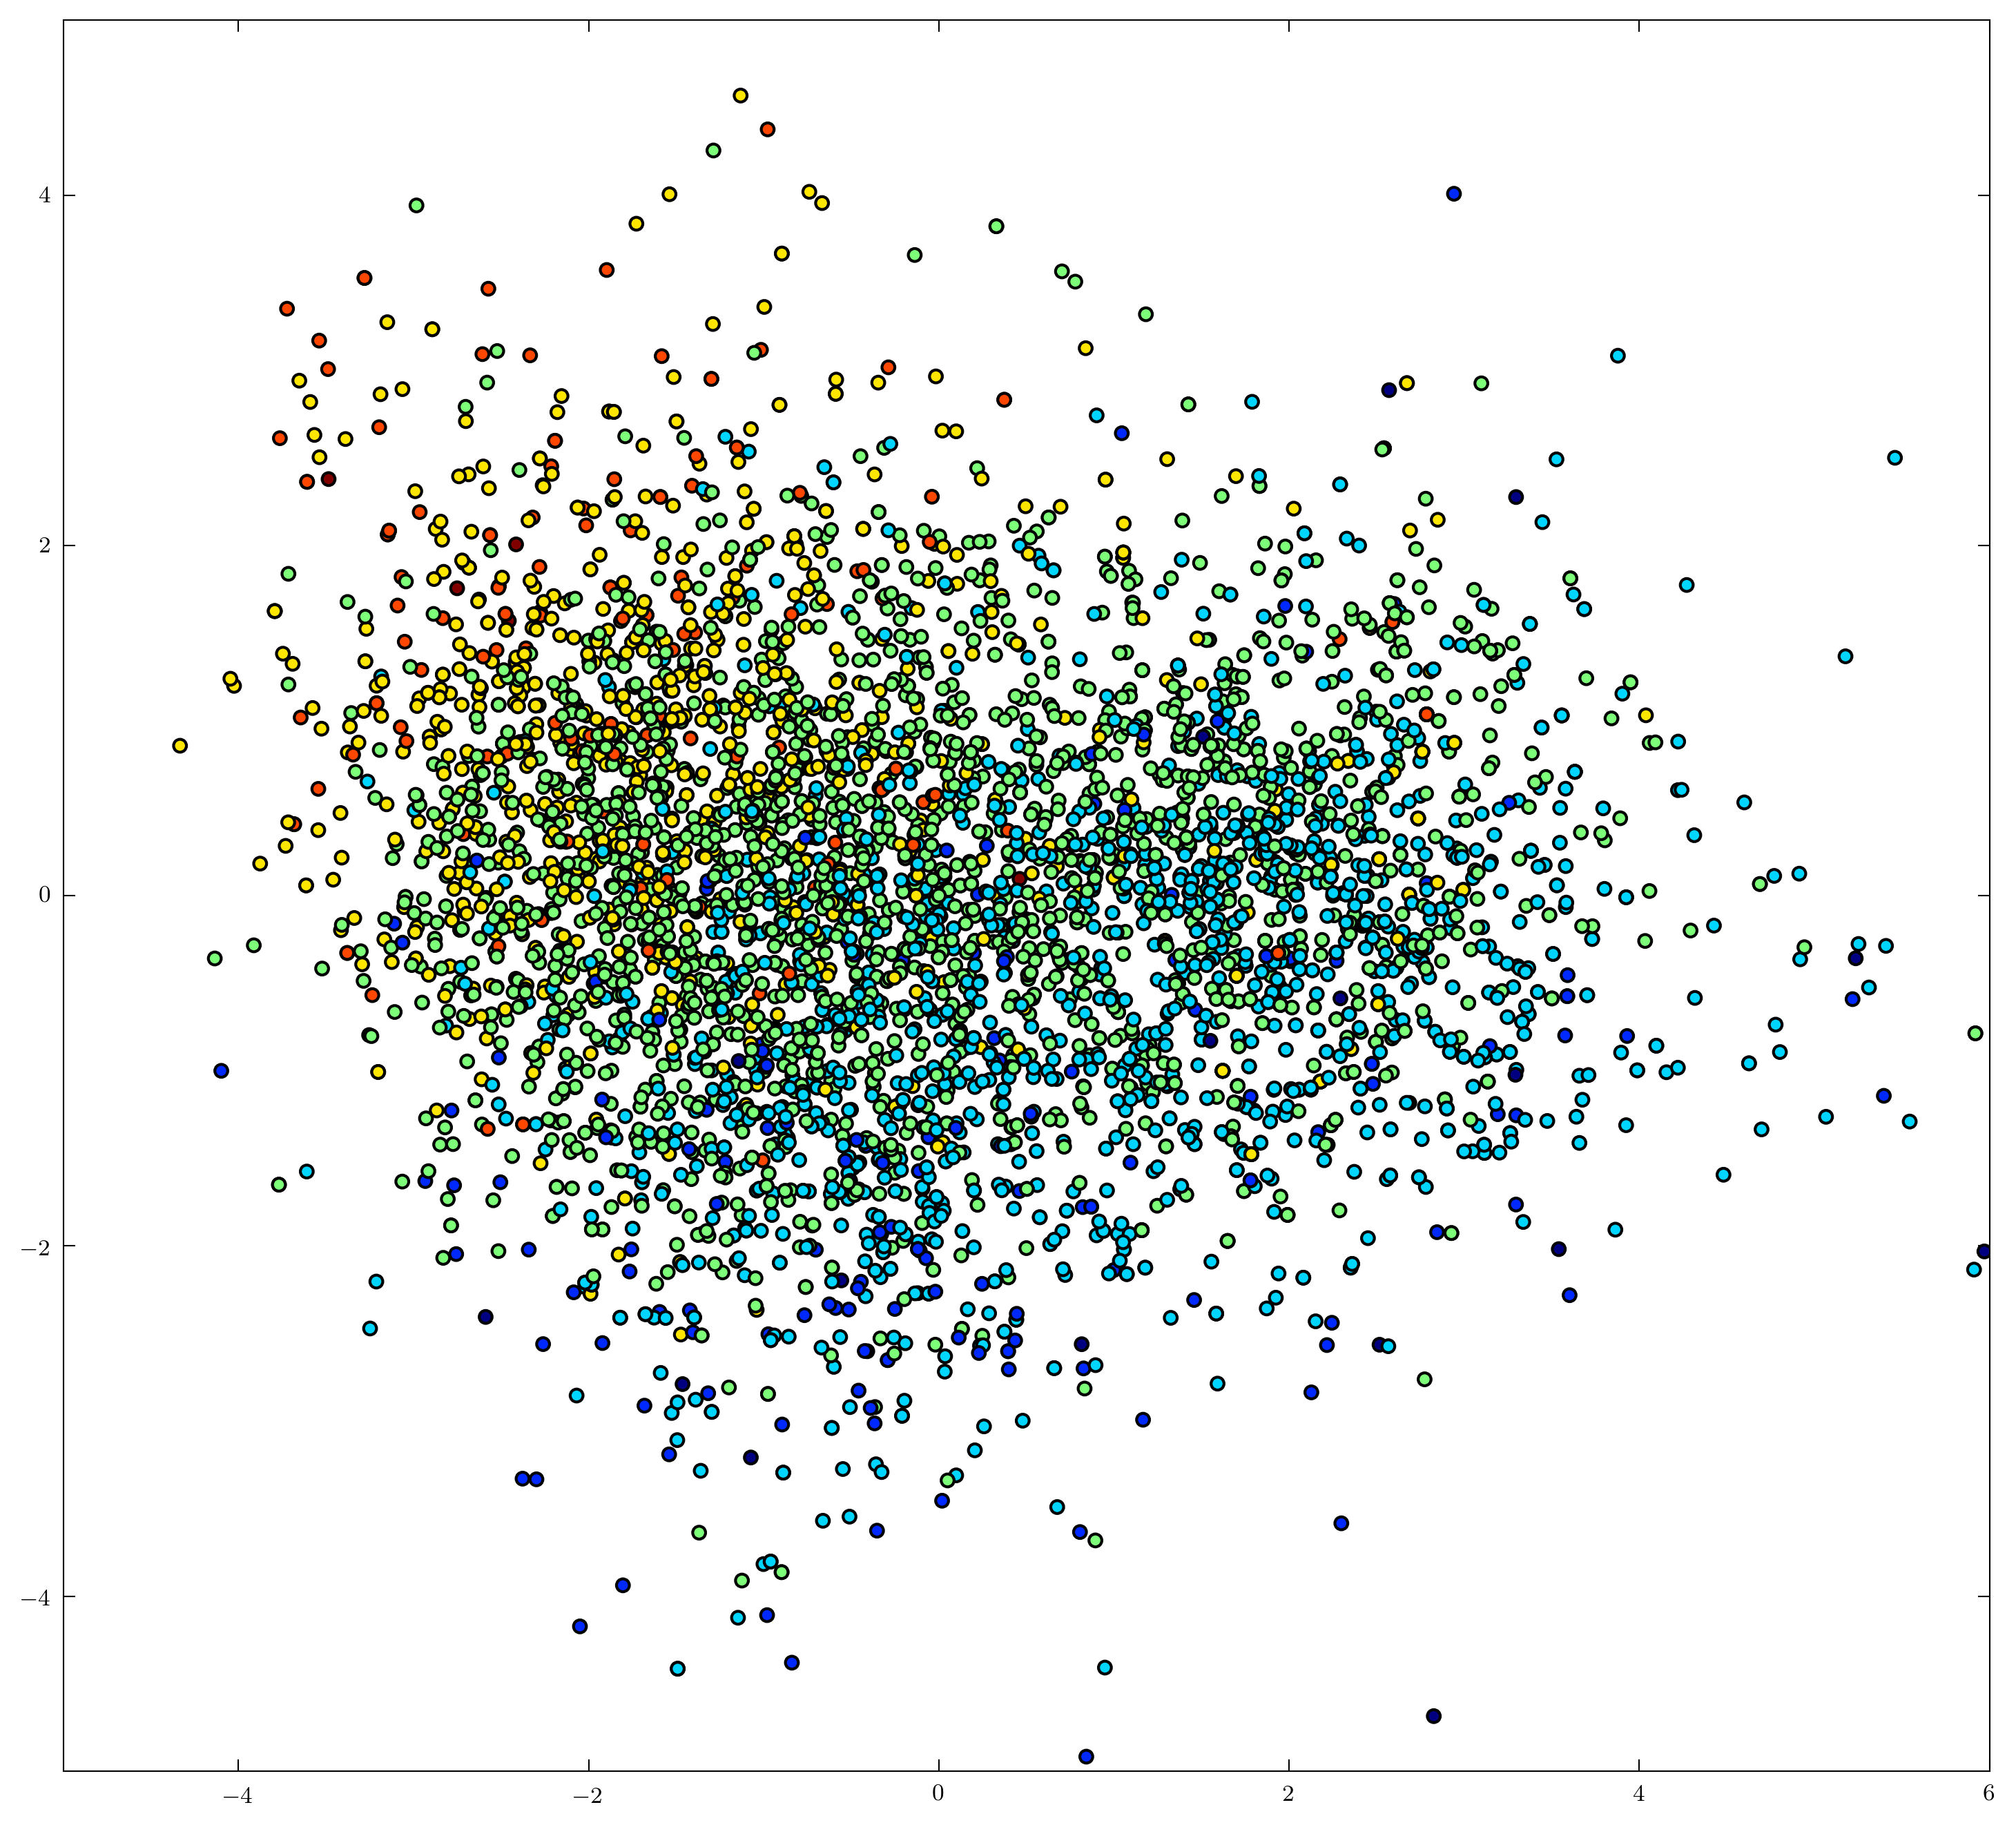
\includegraphics[width=\textwidth]{mds.png}
\caption{2D projection of the normalized data set using MDS with 25 iterations and objective function $E_1$}
\label{mds}
\end{figure}

\newpage

\section{Correlation coefficients using different functions}
\label{ccs}
Based on both the correlation coefficients and the scatter matrices presented before, there seem to be little correlations between the features. Density has some strong correlations with amount of alcohol and residual sugar, but this is to be expected since there sugar is consumed when alcohol is produced, and water is denser than alcohol.

In all the tables below, correlation coefficients with absolute value larger than 0.5 have been emphasized.
\subsection{Correlation coefficients using Pearson's correlation coefficient}
\begin{adjustbox}{max width=\textwidth}
\begin{tabular}{l || *{12}{P{1.2cm}}}
& citric acid & free sulfur dioxide & total sulfur dioxide & alcohol & volatile acidity & sulphates & residual sugar & pH & fixed acidity & density & quality & chlorides\\
\hline 
citric acid & \bftab 1.0000 & 0.0941 & 0.1211 & --0.0757 & --0.1495 & 0.0623 & 0.0942 & --0.1637 & 0.2892 & 0.1495 & --0.0092 & 0.1144 \\

free sulfur dioxide & 0.0941 & \bftab 1.0000 & \bftab 0.6155 & --0.2501 & --0.0970 & 0.0592 & 0.2991 & --0.0006 & --0.0494 & 0.2942 & 0.0082 & 0.1014 \\

total sulfur dioxide & 0.1211 & \bftab 0.6155 & \bftab 1.0000 & --0.4489 & 0.0893 & 0.1346 & 0.4014 & 0.0023 & 0.0911 & \bftab 0.5299 & --0.1747 & 0.1989 \\

alcohol & --0.0757 & --0.2501 & --0.4489 & \bftab 1.0000 & 0.0677 & --0.0174 & --0.4506 & 0.1214 & --0.1209 & \bftab --0.7801 & 0.4356 & --0.3602 \\

volatile acidity & --0.1495 & --0.0970 & 0.0893 & 0.0677 & \bftab 1.0000 & --0.0357 & 0.0643 & --0.0319 & --0.0227 & 0.0271 & --0.1947 & 0.0705 \\

sulphates & 0.0623 & 0.0592 & 0.1346 & --0.0174 & --0.0357 & \bftab 1.0000 & --0.0267 & 0.1560 & --0.0171 & 0.0745 & 0.0537 & 0.0168 \\

residual sugar & 0.0942 & 0.2991 & 0.4014 & --0.4506 & 0.0643 & --0.0267 & \bftab 1.0000 & --0.1941 & 0.0890 & \bftab 0.8390 & --0.0976 & 0.0887 \\

pH & --0.1637 & --0.0006 & 0.0023 & 0.1214 & --0.0319 & 0.1560 & --0.1941 & \bftab 1.0000 & --0.4259 & --0.0936 & 0.0994 & --0.0904 \\

fixed acidity & 0.2892 & --0.0494 & 0.0911 & --0.1209 & --0.0227 & --0.0171 & 0.0890 & --0.4259 & \bftab 1.0000 & 0.2653 & --0.1137 & 0.0231 \\

density & 0.1495 & 0.2942 & \bftab 0.5299 & \bftab --0.7801 & 0.0271 & 0.0745 & \bftab 0.8390 & --0.0936 & 0.2653 & \bftab 1.0000 & --0.3071 & 0.2572 \\

quality & --0.0092 & 0.0082 & --0.1747 & 0.4356 & --0.1947 & 0.0537 & --0.0976 & 0.0994 & --0.1137 & --0.3071 & \bftab 1.0000 & --0.2099 \\

chlorides & 0.1144 & 0.1014 & 0.1989 & --0.3602 & 0.0705 & 0.0168 & 0.0887 & --0.0904 & 0.0231 & 0.2572 & --0.2099 & \bftab 1.0000 \\
\end{tabular}
\end{adjustbox}
\subsection{Correlation coefficients using Spearman's rho}
\begin{adjustbox}{max width=\textwidth}
\begin{tabular}{l || *{12}{P{1.2cm}}}
& citric acid & free sulfur dioxide & total sulfur dioxide & alcohol & volatile acidity & sulphates & residual sugar & pH & fixed acidity & density & quality & chlorides\\
\hline 
citric acid & \bftab 1.0000 & 0.0883 & 0.0932 & --0.0292 & --0.1504 & 0.0798 & 0.0246 & --0.1462 & 0.2979 & 0.0914 & 0.0183 & 0.0327 \\

free sulfur dioxide & 0.0883 & \bftab 1.0000 & \bftab 0.6186 & --0.2726 & --0.0812 & 0.0523 & 0.3461 & --0.0063 & --0.0245 & 0.3278 & 0.0237 & 0.1670 \\

total sulfur dioxide & 0.0932 & \bftab 0.6186 & \bftab 1.0000 & --0.4766 & 0.1176 & 0.1578 & 0.4313 & --0.0118 & 0.1126 & \bftab 0.5638 & --0.1967 & 0.3752 \\

alcohol & --0.0292 & --0.2726 & --0.4766 & \bftab 1.0000 & 0.0340 & --0.0449 & --0.4453 & 0.1489 & --0.1068 & \bftab --0.8219 & 0.4404 & \bftab --0.5708 \\

volatile acidity & --0.1504 & --0.0812 & 0.1176 & 0.0340 & \bftab 1.0000 & --0.0169 & 0.1086 & --0.0452 & --0.0429 & 0.0101 & --0.1966 & --0.0049 \\

sulphates & 0.0798 & 0.0523 & 0.1578 & --0.0449 & --0.0169 & \bftab 1.0000 & --0.0038 & 0.1402 & --0.0132 & 0.0951 & 0.0333 & 0.0939 \\

residual sugar & 0.0246 & 0.3461 & 0.4313 & --0.4453 & 0.1086 & --0.0038 & \bftab 1.0000 & --0.1800 & 0.1067 & \bftab 0.7804 & --0.0821 & 0.2278 \\

pH & --0.1462 & --0.0063 & --0.0118 & 0.1489 & --0.0452 & 0.1402 & --0.1800 & \bftab 1.0000 & --0.4183 & --0.1101 & 0.1094 & --0.0540 \\

fixed acidity & 0.2979 & --0.0245 & 0.1126 & --0.1068 & --0.0429 & --0.0132 & 0.1067 & --0.4183 & \bftab 1.0000 & 0.2700 & --0.0845 & 0.0947 \\

density & 0.0914 & 0.3278 & \bftab 0.5638 & \bftab --0.8219 & 0.0101 & 0.0951 & \bftab 0.7804 & --0.1101 & 0.2700 & \bftab 1.0000 & --0.3484 & \bftab 0.5083 \\

quality & 0.0183 & 0.0237 & --0.1967 & 0.4404 & --0.1966 & 0.0333 & --0.0821 & 0.1094 & --0.0845 & --0.3484 & \bftab 1.0000 & --0.3145 \\

chlorides & 0.0327 & 0.1670 & 0.3752 & \bftab --0.5708 & --0.0049 & 0.0939 & 0.2278 & --0.0540 & 0.0947 & \bftab 0.5083 & --0.3145 & \bftab 1.0000 \\
\end{tabular}
\end{adjustbox}
\subsection{Correlation coefficients using Kendall's tau}
\begin{adjustbox}{max width=\textwidth}
\begin{tabular}{l || *{12}{P{1.2cm}}}
& citric acid & free sulfur dioxide & total sulfur dioxide & alcohol & volatile acidity & sulphates & residual sugar & pH & fixed acidity & density & quality & chlorides\\
\hline 
citric acid & \bftab 1.0000 & 0.0608 & 0.0622 & --0.0200 & --0.1040 & 0.0545 & 0.0153 & --0.1013 & 0.2086 & 0.0615 & 0.0146 & 0.0223 \\

free sulfur dioxide & 0.0608 & \bftab 1.0000 & 0.4447 & --0.1825 & --0.0548 & 0.0356 & 0.2367 & --0.0052 & --0.0169 & 0.2173 & 0.0172 & 0.1139 \\

total sulfur dioxide & 0.0622 & 0.4447 & \bftab 1.0000 & --0.3258 & 0.0813 & 0.1087 & 0.2933 & --0.0084 & 0.0773 & 0.3884 & --0.1512 & 0.2571 \\

alcohol & --0.0200 & --0.1825 & --0.3258 & \bftab 1.0000 & 0.0235 & --0.0264 & --0.3056 & 0.1026 & --0.0732 & \bftab --0.6351 & 0.3467 & --0.4040 \\

volatile acidity & --0.1040 & --0.0548 & 0.0813 & 0.0235 & \bftab 1.0000 & --0.0116 & 0.0728 & --0.0304 & --0.0296 & 0.0066 & --0.1548 & --0.0035 \\

sulphates & 0.0545 & 0.0356 & 0.1087 & --0.0264 & --0.0116 & \bftab 1.0000 & --0.0025 & 0.0958 & --0.0087 & 0.0642 & 0.0264 & 0.0626 \\

residual sugar & 0.0153 & 0.2367 & 0.2933 & --0.3056 & 0.0728 & --0.0025 & \bftab 1.0000 & --0.1256 & 0.0749 & \bftab 0.5890 & --0.0631 & 0.1553 \\

pH & --0.1013 & --0.0052 & --0.0084 & 0.1026 & --0.0304 & 0.0958 & --0.1256 & \bftab 1.0000 & --0.2948 & --0.0756 & 0.0844 & --0.0379 \\

fixed acidity & 0.2086 & --0.0169 & 0.0773 & --0.0732 & --0.0296 & --0.0087 & 0.0749 & --0.2948 & \bftab 1.0000 & 0.1855 & --0.0655 & 0.0654 \\

density & 0.0615 & 0.2173 & 0.3884 & \bftab --0.6351 & 0.0066 & 0.0642 & \bftab 0.5890 & --0.0756 & 0.1855 & \bftab 1.0000 & --0.2666 & 0.3491 \\

quality & 0.0146 & 0.0172 & --0.1512 & 0.3467 & --0.1548 & 0.0264 & --0.0631 & 0.0844 & --0.0655 & --0.2666 & \bftab 1.0000 & --0.2449 \\

chlorides & 0.0223 & 0.1139 & 0.2571 & --0.4040 & --0.0035 & 0.0626 & 0.1553 & --0.0379 & 0.0654 & 0.3491 & --0.2449 & \bftab 1.0000 \\
\end{tabular}
\end{adjustbox}
\end{document}